The goal of this chapter is to make further progress on describing permutation grid classes. In Chapter~\ref{chap:catalanjuxt}, we focused on exact enumeration of a specific set of permutation grid classes of the form $\C|\M$, where $\C$ is a Catalan class, $\M$ is a monotone class, and the gridding is right-most. In this chapter, we trade some amount of ``exactness'' for more generality. In particular, we address permutation grid classes of the form $\M_1|\ldots|\M_k|\C|\M_{k+1}|,\ldots|\M_{k+\ell}$, for some $k,\ell \geq 0$, where $\C$ is an arbitrary \emph{context-free} permutation class. We define what context-free means in Section~\ref{sec:iterjuxt_intro}. For now, let us note that ``Context-free'' is significantly more general than ``Catalan'', yet well-behaved enough to deal with. As opposed to the Catalan classes, we do not enumerate all these context-free juxtapositions exactly as there are infinitely many of them (compare that to the six Catalan juxtapositions) and they could be very disparate. In principle though, our method allows us to enumerate each one of such classes individually. However, exact enumeration is a mere side-product. Instead, we focus on proving that the permutation classes of the form $\M_1|\ldots|\M_k|\C|\M_{k+1}|\ldots|\M_{k+\ell}$ admit algebraic generating functions.

Algebraicity follows from the context-free property of the class itself. In fact, \emph{context-freeness} is what we work with and exploit. Algebraicity of the generating function is a consequence of it. Still, notice that algebraic generating functions are as ``nice'' as one can hope for given that many generating functions enumerating context-free classes are already algebraic and non-rational. Below is a hierarchy of families of generating functions showing that the family of algebraic power series is one of the more special ones.

$$\text{rational} \subset \text{algebraic} \subset \text{$D$-finite} \subset \text{$D$-algebraic} \subset \text{power series}$$

From this viewpoint, our result states that by appending an arbitrary but finite number of monotone classes on either side of a context-free class $\C$, the resulting class does not lose context-freeness and its generating function does not get qualitatively worse compared to the one enumerating $\C$. A notable corollary of this result is, for instance, that juxtaposition of monotone classes on either side of a permutation class $\C$ with finitely many simple permutations admits an algebraic generating function. This is a significant subcase and classes with finitely many simples were studied in e.g.~\cite{albertatkinsonrestricted} and~\cite{brignall2008simple}. Moreover, we work out several examples explicitly to obtain exact generating functions. These are $\Av(321|21)$ (enumerated in Chapter~\ref{chap:catalanjuxt} by a different method), $\M|\M|\M$ from~\cite{bevan2015thesis}, and $\S|\M$ (separable next to monotone).

%The first example is significant in that it shows that not all context-free classes that meet our requirements have finitely many simple permutations. Therefore, the corollary above is actually weaker than our main result. 

\section{Introduction, definitions, prerequisites}
\label{sec:iterjuxt_intro}

To begin, we juxtapose a context-free permutation class $\C$ with a finite row of monotone classes $\M_1|\ldots|\M_k$ on the right. Additionally, we assume for the moment that each
$\M_i$ is monotone and increasing. We later argue that for decreasing classes, a symmetry of our argument applies and renders the case essentially identical to monotone increasing $\M$. We also show that by extending our original arguments, we can handle appending $\M$ on both sides: the left-hand side and the right-hand side of $\C$. So eventually without loss of generality, we append only increasing $\M$ and only from the right --- at least for now. As mentioned above, the work in this chapter extends the work in Chapter~\ref{chap:catalanjuxt} in two directions. One, the condition that $\C$ is a Catalan permutation class is replaced by requiring $\C$ to only be context-free. Two, juxtaposition from the right is iterated a finite number of times instead of just once. Before we proceed with the statement of the result, let us set the scene. The following definition is taken from Flajolet and Sedgewick~\cite{analcomb}, Section I.5.4, Definition I.13.
\begin{definition}[Context-free specification]
  A class $\C$ is said to be \emph{context-free} if it coincides with the first component $\S_1$ of a system of equations
  \begin{align}
  \begin{aligned}
    \begin{cases}
      \S_1 &= f_1(\Z,\S_1,\ldots,\S_r)\\
      &\vdots\\
      \S_r &= f_r(\Z,\S_1,\ldots,\S_r)
    \end{cases}
  \end{aligned}
  \end{align}
  where each $f_i$ is a constructor that only involves operations of combinatorial sum ($+$) and cartesian product ($\times$), as well as the neutral/empty class $\EE = \{\emptyset\}$.
\end{definition}
For our purposes, two classes are the same if there exists a bijection between them. The following definition implies this.
\begin{definition}
  Two combinatorial classes are \emph{combinatorially isomorphic} if and only if their counting sequences are identical. This is equivalent to the existence of a size-preserving bijection between the two classes.
\end{definition}

Before we proceed to modify the definition of a context-free class, we state the key result of Chomsky and Schutzenberger as Theorem~\ref{thm:chomsky}. It relates the character of the class's context-free combinatorial specification to the character of the class' generating function. If the former is ``nice'', then so is the latter. Our work then consists of proving that the juxtaposition classes in question have ``nice'' combinatorial specifications. Once that is known, Theorem~\ref{thm:chomsky} translates the result into the language of generating functions.

\begin{theorem}[Chomsky-Schutzenberger, Proposition I.7. in~\cite{analcomb}]
\label{thm:chomsky}
A combinatorial class $\C$ that is context-free admits an ordinary generating function that is an algebraic function. In other words, there exists a (non-null) bivariate polynomial $P(z,y) \in \mathbb{C}[z,y]$ such that $$P(z,C(z)) = 0.$$
\end{theorem}

As mentioned, we are going to need a modification of the definition of a context-free class that will allow us to decorate context-free permutation classes. 
\begin{definition}[Tracking the left-most and the right-most points]
  We say that a context-free specification of $\C$ \emph{tracks the right-most and the left-most point by vertical position} if it is combinatorialy isomorphic to the context-free class with the specification $\rS$ in~\eqref{eq:combspecS} and all Cartesian products in $\rS$ are recorded left-to-right as they occur bottom-to-top in $\C$. The asterisk (${}^*$) [circle (${}^\circ$)] in $\rS$ mark the right-most [left-most] point, or the block which contains the right-most [left-most] point inside $\C_i^*$ [$\C_i^\circ$]. Notice that a class can contain both the left-most and the right-most point, e.g.~$\C^{\circ*}$. Analogously, we use four different atoms to describe permutation points: the usual point $\Z$, the rightmost point $\Zstar$, the leftmost point $\Z^\circ$, and the rightmost point that is also leftmost, $\Z^{\circ*}$. 
  \begin{align}
\rS &=  \begin{rcases}\begin{dcases}
  \C_0^* &= f_0^*(\Z,\Z^*,\C_i, \C_i^*)\\
       &\vdots\\
  \C_r^* &= f_r^*(\Z,\Z^*,\C_i, \C_i^*)\\
  \C_0^\circ &= f_0^\circ(\Z,\Z^\circ,\C_i,\C_i^\circ)\\
       &\vdots\\
  \C_r^\circ &= f_r^\circ(\Z,\Z^\circ,\C_i, \C_i^\circ)\\
  \C_0^{\circ*} &= f_0^{\circ*}(\Z,\Z^*,\Z^\circ,\Z^{\circ *}, \C_i, \C_i^*,\C_i^\circ, \C_i^{\circ *})\\
       &\vdots\\
  \C_r^{\circ*} &= f_r^{\circ*}(\Z,\Z^*,\Z^\circ,\Z^{\circ *}, \C_i, \C_i^*,\C_i^\circ, \C_i^{\circ *})\\
  \C_0 &= f_0(\Z,\C_0,\ldots,\C_r)\\
       &\vdots\\
  \C_r &= f_r(\Z,\C_0,\ldots,\C_r)
       \end{dcases}
     \end{rcases}
         \label{eq:combspecS}
  \end{align}
  where $0 \leq i \leq r$. 
 \end{definition}

 If a class $\C^*$ tracks the right-most point as outlined above, we refer to $\C^*$ as a \emph{starred class}. Similarly, $\Z^*$ is a \emph{starred point}, or simply the right-most point. Analogously, we have a \emph{circled class} $\C^\circ$ and a \emph{circled point} $\Z^\circ$. On the other hand, we will also use the terms \emph{starless class} or \emph{starless point} to refer to a class without a star/asterisk. For example, $\C, \C^\circ$ and $\Z, \Z^\circ$. Given the above definition, we assume from now on that every permutation in class $\C$ is context-free and admits a specification that tracks the right-most point. When we need to track the left-most point we declare it explicitly.

   
The Cartesian product is naturally non-commutative which conveniently helps us to keep track of vertical positions. Therefore, requiring that the combinatorial specification keeps track of the rightmost point by its value amounts to merely picking a specific combinatorial specification according to how it happens to encode the right-most point in $\C$. 

Let us consider an example of how vertical order translates into left-to-right order in the Cartesian product. For instance, $\Z\C\C\DD$ refers to a term which has a single point at the bottom, then somewhere above it (and to the left or to the right of it) there is an element from $\C$, then another element of $\C$ is further above the previous one, and above all of this there is an element from $\DD$. Schematically, it could look something like the class in Figure~\ref{fig:order}.

\begin{figure}[ht]
  \centering
  \begin{tikzpicture}
    \draw (-0.5,0.5) rectangle (0.5,1.5) node[pos=0.5]{$\DD$};
    \draw (-3,-0.5) rectangle (-2,0.5) node[pos=0.5]{$\C$};
    \draw (-1.5,-1.5) rectangle (-0.5,-0.5) node[pos=0.5]{$\C$};
    \filldraw[black] (-2,-2) circle (2pt);
    \draw (-1.6,-2.2) node {$\Z$};
  \end{tikzpicture}
  \caption{An example of a class which would correspond to a term $\Z\C\C\DD$ in a combinatorial specification that preserves the vertical (bottom-to-top) order of elements.}
  \label{fig:order}
\end{figure}


\begin{example}
  \label{ex:separable_combspec}
  The following is a context-free specification for the class of separable permutations (non-empty):
  \begin{align*}
    \S &= \Z + \S_{\oplus}\S + \S_{\ominus}\S\\
    \S_{\ominus} &= \Z + \S_\oplus\S\\
    \S_\oplus &= \Z + \S_\ominus\S,
  \end{align*}
  where we use $\S_\ominus$ and $\S_\oplus$ to denote the skew-indecomposable and sum-indecomposable permutation classes. Now, among all context-free specifications of $\S$, we insist on picking the following one to track the rightmost point:
  \begin{align}
    \begin{aligned}
    \S^* &= \Z^* + \S_{\oplus}\S^* + \S^*\S_{\ominus}\\
    \S &= \Z + \S_{\oplus}\S + \S\S_{\ominus}\\
    \S_{\ominus} &= \Z + \S_\oplus\S\\
    \S_\oplus &= \Z + \S\S_\ominus.
    \label{eq:sepstarcs}
  \end{aligned}
  \end{align}
  In~\eqref{eq:sepstarcs}, the class of separable permutations is represented according to the decomposition in~\eqref{eq:sepstar}, encoding vertical order as left-to-right. Notice, in particular, that there are multiple combinatorial specifications of $\S$ that track the right-most points. The correctness of the one we chose is clearer in the following schematic diagram.
  \begin{align}
    \begin{aligned}
      \S^* &= \Z + \cplusc{\S_\oplus}{\S^*} + \cminusc{\S^*}{\S_\ominus}\\
      \S &= \Z + \cplusc{\S_\oplus}{\S} + \cminusc{\S}{\S_\ominus}\\
      \S_\ominus &= \Z + \cplusc{\S_\oplus}{\S}\\
      \S_\oplus &= \Z + \cminusc{\S}{\S_\ominus}
    \end{aligned}
                  \label{eq:sepstar}
  \end{align}

Another combinatorial specification of $\S$ that tracks the rightmost point is the following one.
  \begin{align*}
    \S^* &= \Z^* + \cplusc{\S}{\S_\oplus^*} + \cminusc{\S_\ominus^*}{\S}\\
    \S_\ominus^* &= \Z^* + \cplusc{\S}{\S_\oplus^*}\\
    \S_\oplus^* &= \Z^* + \cminusc{\S_\ominus^*}{\S}\\
    \S &= \Z + \cplusc{\S}{\S_\oplus} + \cminusc{\S_\ominus}{\S}\\
    \S_\ominus &= \Z + \cplusc{\S}{\S_\oplus}\\
    \S_\oplus &= \Z + \cminusc{\S_\ominus}{\S}
  \end{align*}
  You will have noticed that we needed to define $\S_\ominus^*$ and $\S_\oplus^*$ in order for this second specification to be closed. That is why, in Section~\ref{sec:example_sepav21}, we prefer to work with~\eqref{eq:sepstar} instead.
\end{example}


Moving from Example~\ref{ex:separable_combspec} back to the general setting, let
$$\V = \{\Z,\Z^*,\C_0,\ldots,\C_r,\C^*_0,\ldots,\C_r^*, \C^\circ_0,\ldots,\C_r^\circ, \C^{\circ*}_0,\ldots,\C_r^{\circ*}\}$$
be the collection of all variables occurring in the polynomials $f_i,f_i^*,f_i^\circ$, and $f_i^{\circ*}$. When we do not care to distinguish between $f_i$ and $f_j$ or $f_i, f_i^*, f_i^\circ$, and $f_i^{\circ*}$, we simply write $f$ for a polynomial in variables from $\V$. Similarly, when we do not distinguish between two variables in $\V$, we simply write $X \in \V$. As we just mentioned, each $f$ is a polynomial. We refer to its terms by $\T_h$ as in $f = \sum_{h=0}^N\T_h$. Each term $\T_h$ is a product of the variables in $\V$ and for a function $f^*$, each $\T_h$ contains exactly one starred variable (there is exactly one rightmost point in each term). The same holds for $f^\circ$. 

One of the problems of enumerating permutation grid classes is that there are often multiple legal ways to grid a permutation in a given grid class. Therefore, one of the key issues we need to address is to choose a particular gridding. We represent every griddable permutation from a juxtaposition by a unique gridded version of it. We pick the gridded version that maximises the element on the right-hand side (RHS) of the juxtaposition. Note that this is a diversion from Chapter~\ref{chap:catalanjuxt}. The following convention makes this concept explicit. See also Figure~\ref{fig:leftmostgridline} for an illustration.
\begin{figure}[ht]
  \centering
  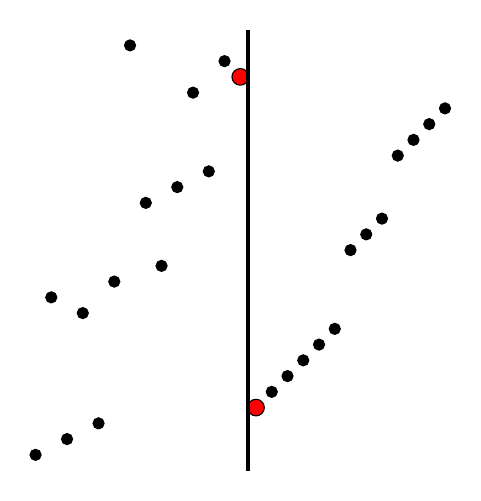
\begin{tikzpicture}[scale=0.2]
\fill[white]  (0,0) rectangle +(27,27);
%\draw[help lines, line width=0.1pt, gray] (0,0) grid +(27,27);
% LHS
\filldraw[black, fill=red] (13.5,24.5) circle (15pt);
\filldraw[black] (12.5,25.5) circle (10pt);
\filldraw[black] (11.5,18.5) circle (10pt);
\filldraw[black] (10.5,23.5) circle (10pt);
\filldraw[black] (9.5,17.5) circle (10pt);
\filldraw[black] (8.5,12.5) circle (10pt);
\filldraw[black] (7.5,16.5) circle (10pt);
\filldraw[black] (6.5,26.5) circle (10pt);
\filldraw[black] (5.5,11.5) circle (10pt);
\filldraw[black] (4.5,2.5) circle (10pt);
\filldraw[black] (3.5,9.5) circle (10pt);
\filldraw[black] (2.5,1.5) circle (10pt);
\filldraw[black] (1.5,10.5) circle (10pt);
\filldraw[black] (.5,.5) circle (10pt);
% RHS
\filldraw[black] (26.5,22.5) circle (10pt);
\filldraw[black] (25.5,21.5) circle (10pt);
\filldraw[black] (24.5,20.5) circle (10pt);
\filldraw[black] (23.5,19.5) circle (10pt);

\filldraw[black] (22.5,15.5) circle (10pt);
\filldraw[black] (21.5,14.5) circle (10pt);
\filldraw[black] (20.5,13.5) circle (10pt);

\filldraw[black] (19.5,8.5) circle (10pt);
\filldraw[black] (18.5,7.5) circle (10pt);
\filldraw[black] (17.5,6.5) circle (10pt);
\filldraw[black] (16.5,5.5) circle (10pt);
\filldraw[black] (15.5,4.5) circle (10pt);
\filldraw[black,fill=red] (14.5,3.5) circle (15pt);
% gridline
\draw[black, line width=0.5mm] (14,-0.5) -- (14,27.5);
\end{tikzpicture}
\caption{\small On the LHS is a permutation from $\C$ while on the RHS is a monotone increasing permutation. The gridline is as far left as possible: if it were shifted further to the left, the red points would form a copy of 21 on the RHS. }
\label{fig:leftmostgridline}
\end{figure}

\noindent\textbf{Convention:} \emph{Let $\pi$ be a permutation from $\C_1|\C_2$. The gridline in $\pi$ is chosen to be the left-most possible. I.e. if it was any further left, the sub-permutation to the right of it would not belong to the designated class $\C_2$.}

The Convention above is a direct consequence of the leftmost gridding. Indeed, let $\C|\M$ be a juxtaposition of any permutation class $\C$ with a monotone increasing permutation class $\M$. Given that the gridline is pushed as far left as possible, the rightmost point in the left cell must be above the leftmost point in the right cell. Otherwise, the gridline could be shifted one more point further left. Figure~\ref{fig:leftmostgridline} shows this well. The left red point must be above the right left point, otherwise the gridline would not have been between these two red points.

Although this will be stated later when needed for Proposition~\ref{prop:leftappend}, dealing with juxtapositions from both sides is quite natural. Given a permutation $\pi$ from $\M_1|\ldots|\M_k|\C|\M_{k+1}|\ldots|\M_{k+\ell}$, we first grid $\ell$ monotone classes from the right according to the Convention. Then flip the picture around a vertical axis and grid the $k$ monotone classes from the right (they used to be on the left), again according to the Convention. Of course, after the flip, we need to treat increasing $\M_i$ as a decreasing class, and vice versa. At the end, the leftover middle part belongs to $\C$. 

We make some further remarks about the way we represent permutations in a juxtaposition. Let $x,y$ be two vertically consecutive points on the left-hand side of the juxtaposition $\C_1|\C_2$. An object on the RHS (e.g. a sequence of points if $\C_2 = \M$) is said to be \emph{associated with} $x$ if it is in the horizontal section of the RHS that falls below $x$ and above $y$. If $x$ is the bottom most point on the LHS, then everything below it on the RHS is associated with $x$. See Figure~\ref{fig:xregion} for an example.
\begin{figure}[ht]
  \centering
  \begin{tikzpicture}
    \filldraw[black] (1,2) circle (2pt) node[above left]{$y$};
    \filldraw[black] (2,4) circle (2pt);
    \filldraw[black] (3,1) circle (2pt);
    \filldraw[black] (4,3) circle (2pt) node[above left]{$x$};
    
    \filldraw[orange, opacity=1] (4.2,0) rectangle (6.3,1);
    \filldraw[orange, opacity=0.66] (4.2,1) rectangle (6.3,2);
    \filldraw[orange, thick, pattern=north west lines, pattern color=orange] (4.2,2) rectangle (6.3,3);
    \filldraw[orange, opacity=0.1] (4.2,3) rectangle (6.3,4);
    \draw[black, line width=0.5mm] (4.1,0) -- (4.1,4.5); % gridline
    \draw[thin] (2.2,4)--(6.5,4);
    \draw[thin] (4.2,3)--(6.5,3);
    \draw[thin] (1.2,2)--(6.5,2);
    \draw[thin] (3.2,1)--(6.5,1);
  \end{tikzpicture}
  \caption{The shaded regions on the RHS each correspond to a gap between two vertically consecutive points on the LHS. The part of the right-hand side associated with $x$ is the hatched region.}
  \label{fig:xregion}
\end{figure}

% Furthermore, to be able to refer to the boxes inside inflations/substitutions by their altitude, we adopt the superscript numbering $\C^j = \C_{\sigma^{-1}(j)}$, meaning that $\C^j$ is inflating the $j$th point of $\sigma$ when counting from bottom to top, i.e. the point $(j,\sigma(j))$ in $\sigma$. Sometimes, we arrange all classes that inflate $\sigma$ in the bottom-to-top order rather than left-to-right. This will be denoted by double square bracket instead of the original single square brackets, i.e. $\sigma\vert{\C^1,\ldots,\C^n}$ means that the order of classes inside bracket is vertical, reading bottom to top. For future use, notice that in left-to-right order, $\C_{|\sigma|}$ refers to the class that inflates the rightmost point of $\sigma$. In vertical order, this class is labelled as $\C^{\sigma(|\sigma|)}$.

Juxtapositions will be expressed via application of operators to context-free classes. We are going to need the following operators: $\Omega_0, \Omega_1, \Omega_\infty, \Omega_{10}, \Omega_{01}, \Omega_{11}$. They represent various forms/stages of juxtaposing a monotone class next to $\C$, in other words, $\Omega_i: \C \mapsto \C'$, where both $\C$ and $\C'$ are context-free permutation classes and $\C'$ is $\C$ with some kind of monotone class next to it on the right. It is important that the property of being context-free is invariant under these operators. Before we present the properties of $\Omega$ operators, we give a short conceptual description of each of them. All of them juxtapose some form of a monotone increasing class to the right of an object (whether a class or a point).
\begin{itemize}
\item[$\Omega_0:$] juxtaposes (interleaves) an empty permutation to the right of a class or a point (i.e. it does nothing except remove the star)
\item[$\Omega_1:$] juxtaposes a single point to the right of a class or a point
\item[$\Omega_\infty:$] juxtaposes an increasing sequence (possibly empty) to the right of a class or a point
\item[$\Omega_{10}:$] juxtaposes an increasing sequence with at least the bottom point, to the right of a class or a point
\item[$\Omega_{01}:$] juxtaposes an increasing sequence with at least the top point, to the right of a class or a point
\item[$\Omega_{11}:$] juxtaposes an increasing sequence with distinct top and bottom points, to the right of a class or a point
\end{itemize}

Furthermore, to ensure we adhere to the convention for gridding, it is desirable that all $\Omega$ operators respect the rightmost point of the class $\C$ they are acting on according to the following rules.
\begin{enumerate}
\item If the operator's code begins with $1$, namely $\Omega_1,\Omega_{10}$, and $\Omega_{11}$, then the operator can only be applied to a starred class, or alternatively, to a starless class occuring before (in left-to-right order) the starred class in the Cartesian product.
\item If the operator's code ends with $0$ or $\infty$, namely $\Omega_0, \Omega_{10}, \Omega_\infty$, then its output is starless. If the operator's code ends with $1$, namely $\Omega_1, \Omega_{01}, \Omega_{11}$, then every term of the output contains exactly one rightmost point (a starred class or point).
\end{enumerate}
Rules 1 and 2 capture the observations that:
\begin{enumerate}
\item If we juxtapose a monotone increasing class next to any class $\C$ to obtain $\C|\M$, then the leftmost/lowest point on the RHS must be below the rightmost point on the LHS. This follows from the Convention as already discussed and even pictured in Figure~\ref{fig:leftmostgridline}.
\item Juxtaposing a class on the right sometimes takes over the rightmost point from the class on the left and it always removes the star from the class on the left. See figures associated with definitions of $\Omega$-operators for examples of when that happens.
\end{enumerate}

Recall that $X_i$ are variables from $\V$. We view every $f$ as a finite sum of terms $\T_h$, each of which is a product of $X_i$s, i.e. $\T_h = X_1X_2\cdots X_m$ for some $m = m(h)$, with all $X_i \in \V$. Without loss of generality, we let $k \in [m]$ be the index of a starred class, i.e. $X_k^*$. In the forthcoming definitions of $\Omega$ operators, let $\C$ be a permutation class that admits a combinatorial specification (combinatorially) isomorphic to $\rS$ in~\eqref{eq:combspecS}. Of course, after applying the $\Omega$-operators, $\rS$ changes its details but not the context-free nature. For example, the set of variables $\V$ will expand as it must now include $\Omega_i(X)$ for some $X$ in the original $\V$.


\noindent\textbf{Operator $\Omega_0$}\\
This operator juxtaposes a class (starred or not) with an empty sequence on the right. Notice, in particular, that $\Omega_0$ distributes over both $+$ and $\times$, and that it erases ${}^*$. 
\begin{align}
  \begin{aligned}
  \Omega_0(\Z) &= \Z\\
  \Omega_0(\Z^*) &= \Z\\
  \Omega_0(\Z^\circ) &= \Z^\circ\\
  \Omega_0(\Z^{\circ*}) &= \Z^{\circ}\\
  \Omega_0(\T_h) = \Omega_0(X_1\cdots X_m) &= \Omega_0(X_1)\Omega_0(X_2\cdots X_m)
\end{aligned}
\end{align}

\noindent\textbf{Operator $\Omega_\infty$}\\
This operator juxtaposes a class (starred or not) with a monotone increasing class -- possibly empty. Again, $\Omega_\infty$ is distributive over operations $+$ and $\times$. As $\Omega_0$, it also erases the ${}^*$. We get the following definition of $\Omega_\infty$. Consult Figure~\ref{fig:omega_infty} with this definition.
\begin{align}
  \begin{aligned}
  \M &= \Z + \M\Z\\
  \Omega_\infty(\Z) &= \M\\
  \Omega_\infty(\Z^*) &= \M\\
  \Omega_\infty(\Z^\circ) &= (\M+\EE)\Z^\circ\\
  \Omega_\infty(\Z^{\circ*}) &= (\M+\EE)\Z^\circ\\
  \Omega_\infty(\T_h) &= \Omega_\infty(X_1)\Omega_\infty(X_2\cdots X_m)
\end{aligned}
                        \label{eq:iterjuxt_omegainfty}
\end{align}
We only include $\M$ to keep the definition self-contained.

\begin{figure}[ht]
  \centering\noindent
    \begin{tikzpicture}
      \filldraw[black] (-5,1) circle (2pt) node[above]{$\Z/\Z^*$};
      \draw[|->] (-4,1)--(-1,1);
      \draw (-2.5,1.3) node{$\Omega_\infty$};
      \filldraw[black] (0,2) circle (2pt);
      \draw (-0.3,2.2) node {$\Z$};
      \draw[-, very thick] (0.2,2.5) -- (0.2,0);
      \draw[dashed] (0.2,2) -- (2.5,2);
      % \filldraw[black] (2.2,1.6) circle (2pt);
      % \draw (2.6,1.6) node {$\Z^*$};
      \draw (1,0.5) rectangle (2,1.5) node[pos=0.5]{$\M^\EE$};
    \end{tikzpicture}
    \begin{tikzpicture}
      \filldraw[black] (-5,1) circle (2pt) node[above]{$\Z^\circ/\Z^{\circ*}$};
      \draw[|->] (-4,1)--(-1,1);
      \draw (-2.5,1.3) node{$\Omega_\infty$};
      \filldraw[black] (0,2) circle (2pt);
      \draw (-0.3,2.2) node {$\Z^\circ\quad$};
      \draw[-, very thick] (0.2,2.5) -- (0.2,0);
      \draw[dashed] (0.2,2) -- (2.5,2);
      % \filldraw[black] (2.2,1.6) circle (2pt);
      % \draw (2.6,1.6) node {$\Z^*$};
      \draw (1,0.5) rectangle (2,1.5) node[pos=0.5]{$\M^\EE$};
    \end{tikzpicture}
    \caption{$\Omega_\infty$: Since $\Omega_\infty$ erases stars, $\Z$ and $\Zstar$ are mapped to the same object. However, $\Z^\circ$ is preserved under all $\Omega$ operators. We denote $\M+\EE$ by $\M^\EE$.}
    \label{fig:omega_infty}
\end{figure}


\noindent\textbf{Operator $\Omega_1$}\\
This operator juxtaposes a class (starred or not) with a single point. It turns out that $\Omega_1$ is linear (over $+$), but does not distribute over $\times$. It either introduces or relocates the right-most point ${}^*$. 
\begin{align}
\begin{aligned}
    \Omega_1(\Z) &= \Z^*\Z\\
    \Omega_1(\Z^*) &= \Z^*\Z\\
    \Omega_1(\Z^\circ) &= \Z^*\Z^\circ\\
    \Omega_1(\Z^{\circ*}) &= \Z^*\Z^\circ\\
  \Omega_1(\T_h) &=
                      \begin{cases}
                        \Omega_1(X_1^*)\Omega_0(X_2\cdots X_m) \quad &\text{if $k = 1$}\\
                        \Omega_1(X_1)\Omega_0(X_2\cdots X_m) + \Omega_0(X_1)\Omega_1(X_2\cdots X_m),\quad &\text{if $k>1$.}
                      \end{cases}
\end{aligned}
\label{eq:iterjuxt_def_omega1}
\end{align}
The base cases ($\Z, \Z^*$ and $\Z^\circ$) are drawn in Figure~\ref{fig:omega_1}. The recursive step $\T_h$ consists of two cases. Either the bottom-most class/point $X_1$ in $\T_h$ is starred (i.e. $X_1 = X_1^*$ or $X_1 = X_1^{\circ*}$) or not. If $X_1^*/X_1^{\circ*}$, then $\Omega_1$ must be applied to it (as it must be applied to a starred class/point or a class/point below it) and $\Omega_0$ is applied to the rest of the classes, $\Omega_0(X_2\cdots X_m)$. If the first class (or point) $X_1$ is not starred, then there are two options. Either apply $\Omega_1$ to $X_1$ and $\Omega_0$ to $X_2\cdots X_m$, or apply $\Omega_0$ to $X_1$ and recursively apply $\Omega_1$ to $X_2\cdots X_m$. Defining operators recursively will be useful when we apply them to permutation classes iteratively.
\begin{figure}[ht]
 \centering
 \begin{tikzpicture}
      \filldraw[black] (-5,1.5) circle (2pt) node[above]{$\Z/\Z^*$};
      \draw[|->] (-4,1.5)--(-1,1.5);
      \draw (-2.5,1.8) node{$\Omega_1$};
%      \filldraw[black] (0,2) circle (2pt);

      \filldraw[black] (0,2) circle (2pt);
      \draw (-0.3,2.2) node {$\Z$};
      \draw[-, very thick] (0.2,2.5) -- (0.2,1);
      \draw[dashed] (0.2,2) -- (2,2);
      \filldraw[black] (1.2,1.6) circle (2pt);
      \draw (1.6,1.6) node {$\Z^*$};
%      \draw (0.5,0.5) rectangle (1.5,1.5) node[pos=0.5]{$\M$};
    \end{tikzpicture}
    \begin{tikzpicture}
      \filldraw[black] (-5,1.5) circle (2pt) node[above]{$\Z^\circ/\Z^{\circ*}$};
      \draw[|->] (-4,1.5)--(-1,1.5);
      \draw (-2.5,1.8) node{$\Omega_1$};
%      \filldraw[black] (0,2) circle (2pt);

      \filldraw[black] (0,2) circle (2pt);
      \draw (-0.3,2.2) node {$\Z^\circ$};
      \draw[-, very thick] (0.2,2.5) -- (0.2,1);
      \draw[dashed] (0.2,2) -- (2,2);
      \filldraw[black] (1.2,1.6) circle (2pt);
      \draw (1.6,1.6) node {$\Z^*$};
%      \draw (0.5,0.5) rectangle (1.5,1.5) node[pos=0.5]{$\M$};
    \end{tikzpicture}
    \caption{$\Omega_1$: Juxtaposing a single point to the right of any point means that the original point is not the right-most anymore and the new one becomes right-most. The left-most point is unafected.}
    \label{fig:omega_1}
\end{figure}

\noindent\textbf{Operator $\Omega_{01}$}\\
This operator juxtaposes a class $\C$ with a monotone sequence that has a distinguished right-most (top-most) point but not the left-most (bottom-most) point. Here, distinguished simply means that we can isolate it from the rest of the points and treat it separately. Recall that this was not the case for $\Omega_\infty$. As usual, $\Omega_{01}$ is linear. It does not distribute over the Cartesian product. Also, $\Omega_{01}$ introduces the right-most point if there was none in $\C/\C^\circ$. Like the rest of the operators, $\Omega_{01}$ does not interact with the left-most point in $\C^\circ/\C^{\circ*}$. See Figure~\ref{fig:omega01}.
\begin{align}
  \begin{aligned}
  \Omega_{01}(\Z) &= (\M+\EE)\Zstar\Z\\
  \Omega_{01}(\Zstar) &= (\M+\EE)\Zstar\Z\\
  \Omega_{01}(\Z^\circ) &= (\M+\EE)\Zstar\Z^\circ\\
  \Omega_{01}(\Z^{\circ*}) &= (\M+\EE)\Zstar\Z^\circ\\
  \Omega_{01}(\T_h) &= \Omega_{01}(X_1)\Omega_0(X_2\cdots X_m)+\Omega_\infty(X_1)\Omega_{01}(X_2\cdots X_m)
\end{aligned}
                      \label{eq:iterjuxt_def_omega01}
\end{align}

\begin{figure}[ht]
 \centering
    \begin{tikzpicture}
      \filldraw[black] (-5,1) circle (2pt) node[above]{$\Z/\Z^*$};
      \draw[|->] (-4,1)--(-1,1);
      \draw (-2.5,1.3) node{$\Omega_{01}$};

      \filldraw[black] (0,2) circle (2pt);
      \draw (-0.3,2.2) node {$\Z$};
      \draw[-, very thick] (0.2,2.5) -- (0.2,0.2);
      \draw[dashed] (0.2,2) -- (2.5,2);
      \filldraw[black] (2.2,1.6) circle (2pt);
      \draw (2.6,1.6) node {$\Z^*$};
      \draw (1,0.5) rectangle (2,1.5) node[pos=0.5]{$\M^\EE$};
    \end{tikzpicture}
    \begin{tikzpicture}
      \filldraw[black] (-5,1) circle (2pt) node[above]{$\Z^\circ/\Z^{\circ*}$};
      \draw[|->] (-4,1)--(-1,1);
      \draw (-2.5,1.3) node{$\Omega_{01}$};

      \filldraw[black] (0,2) circle (2pt);
      \draw (-0.3,2.2) node {$\Z^\circ$};
      \draw[-, very thick] (0.2,2.5) -- (0.2,0.2);
      \draw[dashed] (0.2,2) -- (2.5,2);
      \filldraw[black] (2.2,1.6) circle (2pt);
      \draw (2.6,1.6) node {$\Z^*$};
      \draw (1,0.5) rectangle (2,1.5) node[pos=0.5]{$\M^\EE$};
    \end{tikzpicture}
  \caption{$\Omega_{01}$: Juxtaposing a monotone sequence with tracked right-most point to the right of a point renders that point not right-most (regardless of whether it was or was not before). The right-most point is now the right-most point on the RHS. Also, $\Omega_{01}$ does not affect whether the original point is left-most. We denote $\M+\EE$ by $\M^\EE$.}
  \label{fig:omega01}
\end{figure}

\noindent\textbf{Operator $\Omega_{10}$:}\\
This operator juxtaposes a class $\C$, which might or might not track the left-most and right-most points, with a monotone sequence on the right which has a distinguished left-most (bottom-most) point. Again, $\Omega_{10}$ is linear over $+$. It erases the right-most point from $\Cstar/\C^{\circ*}$ and does not affect the left-most point in $\C^\circ/\C^{\circ*}$. The base cases of the definition below are described in Figures~\ref{fig:omega_10}. 
\begin{align}
  \begin{aligned}
  \Omega_{10}(\Z) &= \Z(\M+\EE)\Z\\
  \Omega_{10}(\Z^*) &= \Z(\M+\EE)\Z\\
  \Omega_{10}(\Z^\circ) &= \Z(\M+\EE)\Z^\circ\\
  \Omega_{10}(\Z^{\circ*}) &= \Z(\M+\EE)\Z^\circ\\
  \Omega_{10}(\T_h) &=
                      \begin{cases}
                        \Omega_{10}(X_1^*)\Omega_\infty(X_2\cdots X_m)  &\text{if $k = 1$}\\
                        \begin{rcases}
                          \Omega_{10}(X_1)\Omega_\infty(X_2\cdots X_m)+\\
                          \quad+\Omega_0(X_1)\Omega_{10}(X_2\cdots X_m)
                        \end{rcases} \quad &\text{if $k>1$.}
                      \end{cases}
                    \end{aligned}
\label{eq:iterjuxt_def_omega10}
\end{align}

\begin{figure}[ht]
    \centering
    \begin{tikzpicture}
      \filldraw[black] (-5,1) circle (2pt) node[above]{$\Z/\Z^*$};
      \draw[|->] (-4,1)--(-1,1);
      \draw (-2.5,1.3) node{$\Omega_{10}$};
      \filldraw[black] (0,2) circle (2pt);
      \draw (-0.3,2.2) node {$\Z$};
      \draw[-, very thick] (0.2,2.5) -- (0.2,0);
      \draw[dashed] (0.2,2) -- (2.5,2);
      % \filldraw[black] (2.2,1.6) circle (2pt);
      % \draw (2.6,1.6) node {$\Z^*$};
      \draw (1,0.5) rectangle (2,1.5) node[pos=0.5]{$\M^\EE$};
      \filldraw[black] (0.8,0.3) circle (2pt);
      \draw (1.2,0.2) node {$\Z$};
    \end{tikzpicture}
    \begin{tikzpicture}
      \filldraw[black] (-5,1) circle (2pt) node[above]{$\Z^\circ/\Z^{\circ*}$};
      \draw[|->] (-4,1)--(-1,1);
      \draw (-2.5,1.3) node{$\Omega_{10}$};
      \filldraw[black] (0,2) circle (2pt);
      \draw (-0.3,2.2) node {$\Z^\circ$};
      \draw[-, very thick] (0.2,2.5) -- (0.2,0);
      \draw[dashed] (0.2,2) -- (2.5,2);
      % \filldraw[black] (2.2,1.6) circle (2pt);
      % \draw (2.6,1.6) node {$\Z^*$};
      \draw (1,0.5) rectangle (2,1.5) node[pos=0.5]{$\M^\EE$};
      \filldraw[black] (0.8,0.3) circle (2pt);
      \draw (1.2,0.2) node {$\Z$};
    \end{tikzpicture}
    \caption{$\Omega_{10}$: Juxtaposing a monotone sequence with tracked left-most point to the right of a point renders that point not right-most (regardless of whether it was or was not before) and does not affect whether that point is left-most. We denote $\M+\EE$ by $\M^\EE$.} 
    \label{fig:omega_10}
  \end{figure}

\noindent\textbf{Operator $\Omega_{11}$:}
This operator juxtaposes a class $\C$, which might or might not track the right-most or left-most points, on the right with a monotone increasing sequence that has both its extremal points distinguished: the left-most point and the rightmost point. As usual, $\Omega_{11}$ is linear over $+$. Also, $\Omega_{11}$ does not affect the left-most point of $\C^\circ/\C^{\circ*}$ and replaces the right-most point of $\Cstar/\C^{\circ*}$. See Figure~\ref{fig:omega11}.
\begin{align}
  \begin{aligned}
  \Omega_{11}(\Z) &= \Z(\M+\EE)\Z^*\Z\\
  \Omega_{11}(\Z^*) &= \Z(\M+\EE)\Z^*\Z\\
  \Omega_{11}(\Z^\circ) &= \Z(\M+\EE)\Z^*\Z^\circ\\
  \Omega_{11}(\Z^{\circ*}) &= \Z(\M+\EE)\Z^*\Z^\circ\\
  \Omega_{11}(\T_h) &=
  \begin{cases}
    \begin{rcases}
      \Omega_{11}(X_1^*)\Omega_0(X_2\cdots X_m)+\ \ \ \\
      \quad+\Omega_{10}(X_1^*)\Omega_{01}(X_2\cdots X_m)\ \ 
    \end{rcases} &\text{if $k = 1$}\\
    \begin{rcases}
      \Omega_{11}(X_1)\Omega_0(X_2\cdots X_m) +\\
      \quad+\Omega_{10}(X_1)\Omega_{01}(X_2\cdots X_m) +\\
      \quad+\Omega_0(X_1)\Omega_{11}(X_2\cdots X_m)
    \end{rcases} &\text{if $k>1$.}
  \end{cases}
\end{aligned}
                   \label{eq:iterjuxt_def_omega11}
\end{align}

\begin{figure}[ht]
 \centering
    \begin{tikzpicture}
      \filldraw[black] (-5,1) circle (2pt) node[above]{$\Z/\Z^*$};
      \draw[|->] (-4,1)--(-1,1);
      \draw (-2.5,1.3) node{$\Omega_{11}$};

      \filldraw[black] (0,2) circle (2pt);
      \draw (-0.3,2.2) node {$\Z$};
      \draw[-, very thick] (0.2,2.5) -- (0.2,0);
      \draw[dashed] (0.2,2) -- (2.5,2);
      \filldraw[black] (2.2,1.6) circle (2pt);
      \draw (2.6,1.6) node {$\Z^*$};
      \draw (1,0.5) rectangle (2,1.5) node[pos=0.5]{$\M^\EE$};
      \filldraw[black] (0.8,0.3) circle (2pt);
      \draw (1.2,0.2) node {$\Z$};
    \end{tikzpicture}
    \begin{tikzpicture}
      \filldraw[black] (-5,1) circle (2pt) node[above]{$\Z^\circ/\Z^{\circ*}$};
      \draw[|->] (-4,1)--(-1,1);
      \draw (-2.5,1.3) node{$\Omega_{11}$};

      \filldraw[black] (0,2) circle (2pt);
      \draw (-0.3,2.2) node {$\Z^\circ$};
      \draw[-, very thick] (0.2,2.5) -- (0.2,0);
      \draw[dashed] (0.2,2) -- (2.5,2);
      \filldraw[black] (2.2,1.6) circle (2pt);
      \draw (2.6,1.6) node {$\Z^*$};
      \draw (1,0.5) rectangle (2,1.5) node[pos=0.5]{$\M^\EE$};
      \filldraw[black] (0.8,0.3) circle (2pt);
      \draw (1.2,0.2) node {$\Z$};
    \end{tikzpicture}
  \caption{$\Omega_{11}$: juxtaposing a monotone sequence with tracked left-most and right-most most points to the right of a single point. The RHS now contains the right-most point whether we started with $\Z,\Zstar,\Z^\circ$ or $\Z^{\circ*}$. The original point was the left-most, this property of it remains unaffected. We denote $\M+\EE$ by $\M^\EE$.}
  \label{fig:omega11}
\end{figure}

To help us with enumeration, we append \emph{phantom} points to permutations or permutation classes. By phantom, we mean a temporary extra point that is not really supposed to be there. The reason we need to do such a thing comes up in the situation portrayed in Figure~\ref{fig:illustrate_phantom_pt}. We said that in a juxtaposition we associate monotone sequences (on the RHS) with points (on the LHS) by placing them into the gaps directly below those points, see Figure~\ref{fig:xregion}. However, in a juxtaposition, the points on the RHS can occur above the top-most point on the LHS as well. So we are one gap short. To remedy this, we add a temporary point to the permutation on the LHS. It is placed above all other points on the LHS and thereby creates the additional gap that we were missing. After applying the operators, we then remove this extra point from our counting expression. Next, we offer a formal definition of a phantom point.
\begin{figure}[ht!]
 \centering
 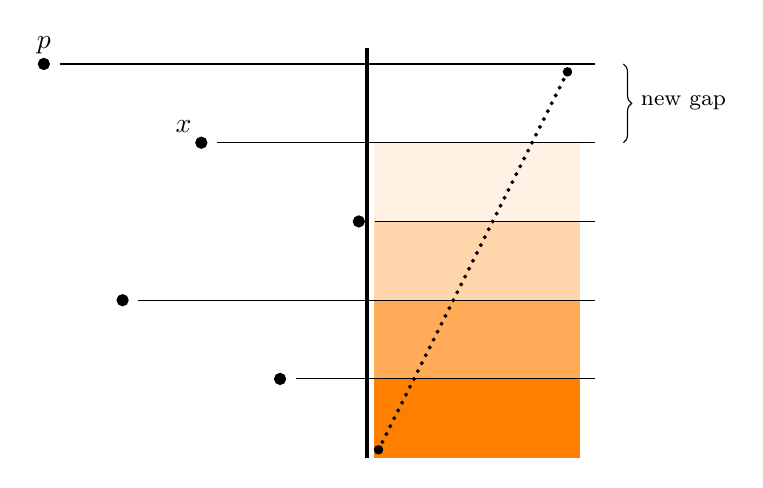
\begin{tikzpicture}
   \filldraw[black] (0,5) circle (2pt) node[above]{$p$};
    \filldraw[black] (1,2) circle (2pt);
    \filldraw[black] (2,4) circle (2pt) node[above left]{$x$};
    \filldraw[black] (3,1) circle (2pt);
    \filldraw[black] (4,3) circle (2pt);
    
    \filldraw[orange, opacity=1] (4.2,0) rectangle (6.8,1);
    \filldraw[orange, opacity=0.66] (4.2,1) rectangle (6.8,2);
    \filldraw[orange, opacity=0.33] (4.2,2) rectangle (6.8,3);
    \filldraw[orange, opacity=0.1] (4.2,3) rectangle (6.8,4);
    \draw[black, line width=0.5mm] (4.1,0) -- (4.1,5.2); % gridline
    \draw[thin] (0.2,5)--(7,5);
    \draw[thin] (2.2,4)--(7,4);
    \draw[thin] (4.2,3)--(7,3);
    \draw[thin] (1.2,2)--(7,2);
    \draw[thin] (3.2,1)--(7,1);
    % sequence on the RHS
    \foreach \i in {1,...,49}
    {
      \filldraw[black] (4.2+0.05*\i,0+0.1*\i) circle (0.5pt);
    }
    \filldraw[black] (4.25,0.1) circle (1.5pt);
    \filldraw[black] (6.65,4.9) circle (1.5pt);

    \draw [decorate,decoration={brace,amplitude=3pt, mirror},xshift=-4pt,yshift=0pt] (7.5,4) -- (7.5,5) node [black, below right, yshift=-8pt]{\footnotesize \ new gap};
  \end{tikzpicture}
  \caption{Compare with Figure~\ref{fig:xregion}. Phantom point $p$ created an extra gap where we can place a monotone sequence --- above the topmost point $x$ of $\pi=2413$. When done with enumeration, it is necessary to remove $p$ as it is not part of $\pi$ and we do not want it to distort the generating function.}
  \label{fig:illustrate_phantom_pt}
\end{figure}

\begin{definition}[Phantom point]
  Let $\pi$ be a permutation from $\C$. An \emph{upper phantom point} $p$ of $\pi$ is a point temporarily added to $\pi$ that has value $|\pi|+1$ and position $0$. In other words, if $\pi'$ denotes $\pi$ with an added upper phantom point, then
  $$\pi' = p \ominus \pi.$$
  We sometimes refer to $\pi$ as an upper phantom point of $\C$, meaning that every $\pi$ in $\C$ is treated as $\pi' = p \ominus \pi$. A \emph{lower phantom point} of $\pi$, usually denoted by $q$, is a point external to $\pi$ that has value $0$ and position $0$. In other words, if $\pi'$ denotes $\pi$ with an added lower phantom point, then
  $$\pi' = q \oplus \pi.$$
We always need only one phantom point at a time and we will always specify which one. If $\C$ is equipped with a phantom point, it is denoted by $\barC$.
\end{definition}
Given that phantom points act as usual points of a permutation, they get acted on by $\Omega$ operators. Exactly as intended. It will become clear why we need the lower phantom point when we append decreasing sequences on the right side of context-free classes.

Before we give an example of how to apply $\Omega_{11}$ and how a phantom point behaves in practice, let us phrase one last observation as a lemma. It will be useful in the forthcoming proofs and examples.

\begin{lemma}
  The following operators ``ignore'' the right-most points (stars) in their arguments as indicated below.
  \begin{enumerate}
  \item $\Omega_0(\Cstar) = \Omega_0(\C) = \C$
  \item $\Omega_\infty(\Cstar) = \Omega_\infty(\C)$
  \item $\Omega_{01}(\Cstar) = \Omega_{01}(\C)$.
  \end{enumerate}
  \label{lem:ignorance}
\end{lemma}
\begin{proof}
First, notice that any term in any polynomial from a context-free specification of some $\C$ remains unaffected by $\Omega_0$. This follows from the definition. Second, again by definition, $\Omega_0$ acts identically on starred and starless objects. This proves the first item. For the same reasons, action of $\Omega_\infty$ and $\Omega_{01}$ does not depend on the rightmost point in the class they take as argument.
\end{proof}


Having defined all necessary concepts, let us consider an example of $\Omega_{11}$ acting on a term $\T_h = X_1X_2X_3^*X_4p = X_1X_2X_3^*X_4\Z$, where $p$ is an upper phantom point. For no particular reason we assume that $X_1X_2X_3X_4$ are classes inflating $2413$. See Figure~\ref{fig:iterjuxt_omega11action} for pictorial representation of the juxtapositions as well as their descriptions in terms of $\Omega$ operators in the captions. We use Lemma~\ref{lem:ignorance} to simplify the expressions by omitting $\Omega_0$ operator, e.g. $\Omega_0(\Z)$ reduces to $\Z$. The first row of Figure~\ref{fig:iterjuxt_omega11action} shows the terms in the recursion which only rely on $\Omega_{11}$ and $\Omega_0$ operators. The remaining terms do not use $\Omega_{11}$, however they additionally employ $\Omega_\infty$, $\Omega_{10}$, and $\Omega_{01}$ operators.

\begin{figure}[!ht]
  \centering
  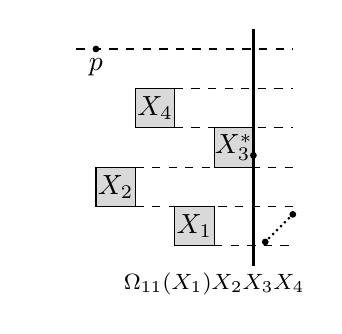
\begin{tikzpicture}[scale=0.5]
    % dashed lines
    \draw[dashed] (2,4) -- (5,4);
    \draw[dashed] (2,3) -- (5,3);
    \draw[dashed] (1,2) -- (5,2);
    \draw[dashed] (1,1) -- (5,1);
    \draw[dashed] (3,0) -- (5,0);
    \draw[dashed] (-0.5,5) -- (5,5); % p-line
%    \draw[dashed] (-2,9) -- (10,9); % q-line
    
    \filldraw[black] (0,5) circle (2pt) node[below]{$p$};
%    \filldraw[black] (-2,9) circle (2pt) node[above]{$q$};
    
    \draw[fill=gray!30] (1,3) rectangle (2,4) node[pos=0.5]{$X_4$};
    \draw[fill=gray!30] (3,2) rectangle (4,3) node[pos=0.5]{$X^*_3$};
    \draw[fill=gray!30] (0,1) rectangle (1,2) node[pos=0.5]{$X_2$};
    \draw[fill=gray!30] (2,0) rectangle (3,1) node[pos=0.5]{$X_1$};
    \draw[-, very thick] (4,-0.5) -- (4,5.5);
    \filldraw[black] (4,2.3) circle (2pt);

    \foreach \i in {1,...,8}
    {
      \filldraw[black] (4.2+0.1*\i,0+0.1*\i) circle (0.5pt);
    }
    \filldraw[black] (4.3,0.1) circle (2pt);
    \filldraw[black] (5.0,0.8) circle (2pt);

    \draw (-1.5,-1) node{};
    \draw (3,-1.5) node[above]{\footnotesize $\Omega_{11}(X_1)X_2X_3X_4\Z$};
  \end{tikzpicture}\hfill
  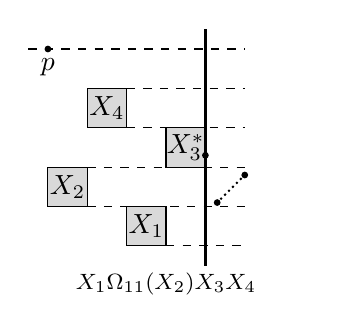
\begin{tikzpicture}[scale=0.5]
    % dashed lines
    \draw[dashed] (2,4) -- (5,4);
    \draw[dashed] (2,3) -- (5,3);
    \draw[dashed] (1,2) -- (5,2);
    \draw[dashed] (1,1) -- (5,1);
    \draw[dashed] (3,0) -- (5,0);
    \draw[dashed] (-0.5,5) -- (5,5); % p-line
%    \draw[dashed] (-2,9) -- (10,9); % q-line
    
    \filldraw[black] (0,5) circle (2pt) node[below]{$p$};
%    \filldraw[black] (-2,9) circle (2pt) node[above]{$q$};
    
    \draw[fill=gray!30] (1,3) rectangle (2,4) node[pos=0.5]{$X_4$};
    \draw[fill=gray!30] (3,2) rectangle (4,3) node[pos=0.5]{$X^*_3$};
    \draw[fill=gray!30] (0,1) rectangle (1,2) node[pos=0.5]{$X_2$};
    \draw[fill=gray!30] (2,0) rectangle (3,1) node[pos=0.5]{$X_1$};
    \draw[-, very thick] (4,-0.5) -- (4,5.5);
    \filldraw[black] (4,2.3) circle (2pt);

    \foreach \i in {1,...,8}
    {
      \filldraw[black] (4.2+0.1*\i,1+0.1*\i) circle (0.5pt);
    }
    \filldraw[black] (4.3,1.1) circle (2pt);
    \filldraw[black] (5.0,1.8) circle (2pt);

    \draw (6.8,-1) node{};
    \draw (3,-1.5) node[above]{\footnotesize $X_1\Omega_{11}(X_2)X_3X_4\Z$};
  \end{tikzpicture}\hfill
  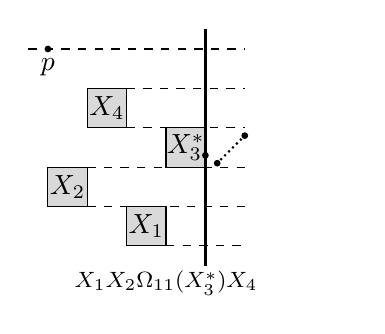
\begin{tikzpicture}[scale=0.5]
    % dashed lines
    \draw[dashed] (2,4) -- (5,4);
    \draw[dashed] (2,3) -- (5,3);
    \draw[dashed] (1,2) -- (5,2);
    \draw[dashed] (1,1) -- (5,1);
    \draw[dashed] (3,0) -- (5,0);
    \draw[dashed] (-0.5,5) -- (5,5); % p-line
%    \draw[dashed] (-2,9) -- (10,9); % q-line
    
    \filldraw[black] (0,5) circle (2pt) node[below]{$p$};
%    \filldraw[black] (-2,9) circle (2pt) node[above]{$q$};
    
    \draw[fill=gray!30] (1,3) rectangle (2,4) node[pos=0.5]{$X_4$};
    \draw[fill=gray!30] (3,2) rectangle (4,3) node[pos=0.5]{$X^*_3$};
    \draw[fill=gray!30] (0,1) rectangle (1,2) node[pos=0.5]{$X_2$};
    \draw[fill=gray!30] (2,0) rectangle (3,1) node[pos=0.5]{$X_1$};
    \draw[-, very thick] (4,-0.5) -- (4,5.5);
    \filldraw[black] (4,2.3) circle (2pt);

    \foreach \i in {1,...,8}
    {
      \filldraw[black] (4.2+0.1*\i,2+0.1*\i) circle (0.5pt);
    }
    \filldraw[black] (4.3,2.1) circle (2pt);
    \filldraw[black] (5.0,2.8) circle (2pt);

    \draw (7.6,-1) node{};
    \draw (3,-1.5) node[above]{\footnotesize $X_1X_2\Omega_{11}(X_3^*)X_4\Z$};
  \end{tikzpicture}\\ \ \\
%\caption{The terms that include $\Omega_{11}$.}
%  \label{fig:iterjuxt_omega11action1}

  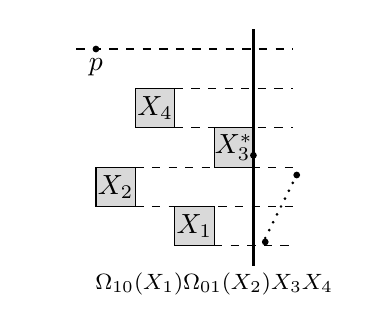
\begin{tikzpicture}[scale=0.5]
    % dashed lines
    \draw[dashed] (2,4) -- (5,4);
    \draw[dashed] (2,3) -- (5,3);
    \draw[dashed] (1,2) -- (5,2);
    \draw[dashed] (1,1) -- (5,1);
    \draw[dashed] (3,0) -- (5,0);
    \draw[dashed] (-0.5,5) -- (5,5); % p-line
%    \draw[dashed] (-2,9) -- (10,9); % q-line
    
    \filldraw[black] (0,5) circle (2pt) node[below]{$p$};
%    \filldraw[black] (-2,9) circle (2pt) node[above]{$q$};
    
    \draw[fill=gray!30] (1,3) rectangle (2,4) node[pos=0.5]{$X_4$};
    \draw[fill=gray!30] (3,2) rectangle (4,3) node[pos=0.5]{$X^*_3$};
    \draw[fill=gray!30] (0,1) rectangle (1,2) node[pos=0.5]{$X_2$};
    \draw[fill=gray!30] (2,0) rectangle (3,1) node[pos=0.5]{$X_1$};
    \draw[-, very thick] (4,-0.5) -- (4,5.5);
    \filldraw[black] (4,2.3) circle (2pt);

    \foreach \i in {1,...,8}
    {
      \filldraw[black] (4.2+0.1*\i,0+0.2*\i) circle (0.5pt);
    }
    \filldraw[black] (4.3,0.1) circle (2pt);
    \filldraw[black] (5.1,1.8) circle (2pt);

    \draw (-1.5,-1) node{};
    \draw (3,-1.5) node[above]{\footnotesize $\Omega_{10}(X_1)\Omega_{01}(X_2)X_3X_4\Z$};
  \end{tikzpicture}\hfill
  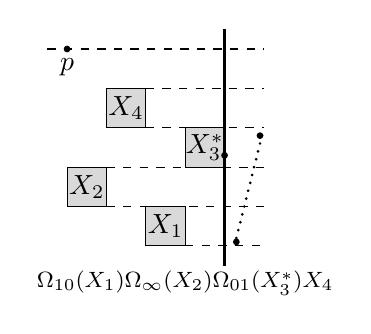
\begin{tikzpicture}[scale=0.5]
    % dashed lines
    \draw[dashed] (2,4) -- (5,4);
    \draw[dashed] (2,3) -- (5,3);
    \draw[dashed] (1,2) -- (5,2);
    \draw[dashed] (1,1) -- (5,1);
    \draw[dashed] (3,0) -- (5,0);
    \draw[dashed] (-0.5,5) -- (5,5); % p-line
%    \draw[dashed] (-2,9) -- (10,9); % q-line
    
    \filldraw[black] (0,5) circle (2pt) node[below]{$p$};
%    \filldraw[black] (-2,9) circle (2pt) node[above]{$q$};
    
    \draw[fill=gray!30] (1,3) rectangle (2,4) node[pos=0.5]{$X_4$};
    \draw[fill=gray!30] (3,2) rectangle (4,3) node[pos=0.5]{$X^*_3$};
    \draw[fill=gray!30] (0,1) rectangle (1,2) node[pos=0.5]{$X_2$};
    \draw[fill=gray!30] (2,0) rectangle (3,1) node[pos=0.5]{$X_1$};
    \draw[-, very thick] (4,-0.5) -- (4,5.5);
    \filldraw[black] (4,2.3) circle (2pt);

    \foreach \i in {1,...,14}
    {
      \filldraw[black] (4.25+0.05*\i,0.2*\i) circle (0.5pt);
    }
    \filldraw[black] (4.3,0.1) circle (2pt);
    \filldraw[black] (4.9,2.8) circle (2pt);

    \draw (3,-1.5) node[above]{\footnotesize $\Omega_{10}(X_1)\Omega_\infty(X_2)\Omega_{01}(X_3^*)X_4\Z$};
  \end{tikzpicture}\hfill
  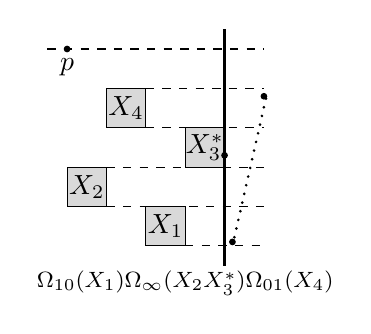
\begin{tikzpicture}[scale=0.5]
    % dashed lines
    \draw[dashed] (2,4) -- (5,4);
    \draw[dashed] (2,3) -- (5,3);
    \draw[dashed] (1,2) -- (5,2);
    \draw[dashed] (1,1) -- (5,1);
    \draw[dashed] (3,0) -- (5,0);
    \draw[dashed] (-0.5,5) -- (5,5); % p-line
%    \draw[dashed] (-2,9) -- (10,9); % q-line
    
    \filldraw[black] (0,5) circle (2pt) node[below]{$p$};
%    \filldraw[black] (-2,9) circle (2pt) node[above]{$q$};
    
    \draw[fill=gray!30] (1,3) rectangle (2,4) node[pos=0.5]{$X_4$};
    \draw[fill=gray!30] (3,2) rectangle (4,3) node[pos=0.5]{$X^*_3$};
    \draw[fill=gray!30] (0,1) rectangle (1,2) node[pos=0.5]{$X_2$};
    \draw[fill=gray!30] (2,0) rectangle (3,1) node[pos=0.5]{$X_1$};
    \draw[-, very thick] (4,-0.5) -- (4,5.5);
    \filldraw[black] (4,2.3) circle (2pt);

    \foreach \i in {1,...,17}
    {
      \filldraw[black] (4.2+0.05*\i,0.22*\i) circle (0.5pt);
    }
    \filldraw[black] (4.2,0.1) circle (2pt);
    \filldraw[black] (5,3.8) circle (2pt);

    \draw (3,-1.5) node[above]{\footnotesize $\Omega_{10}(X_1)\Omega_\infty(X_2X_3^*)\Omega_{01}(X_4)\Z$};
  \end{tikzpicture}\\ \ \\
  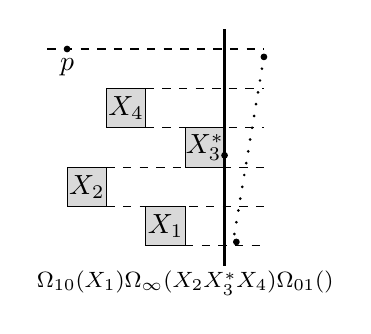
\begin{tikzpicture}[scale=0.5]
    % dashed lines
    \draw[dashed] (2,4) -- (5,4);
    \draw[dashed] (2,3) -- (5,3);
    \draw[dashed] (1,2) -- (5,2);
    \draw[dashed] (1,1) -- (5,1);
    \draw[dashed] (3,0) -- (5,0);
    \draw[dashed] (-0.5,5) -- (5,5); % p-line
%    \draw[dashed] (-2,9) -- (10,9); % q-line
    
    \filldraw[black] (0,5) circle (2pt) node[below]{$p$};
%    \filldraw[black] (-2,9) circle (2pt) node[above]{$q$};
    
    \draw[fill=gray!30] (1,3) rectangle (2,4) node[pos=0.5]{$X_4$};
    \draw[fill=gray!30] (3,2) rectangle (4,3) node[pos=0.5]{$X^*_3$};
    \draw[fill=gray!30] (0,1) rectangle (1,2) node[pos=0.5]{$X_2$};
    \draw[fill=gray!30] (2,0) rectangle (3,1) node[pos=0.5]{$X_1$};
    \draw[-, very thick] (4,-0.5) -- (4,5.5);
    \filldraw[black] (4,2.3) circle (2pt);

    \foreach \i in {1,...,15}
    {
      \filldraw[black] (4.2+0.05*\i,0.3*\i) circle (0.5pt);
    }
    \filldraw[black] (4.3,0.1) circle (2pt);
    \filldraw[black] (5.0,4.8) circle (2pt);

    \draw (3,-1.5) node[above]{\footnotesize $\Omega_{10}(X_1)\Omega_\infty(X_2X_3^*X_4)\Omega_{01}(\Z)$};
  \end{tikzpicture}
  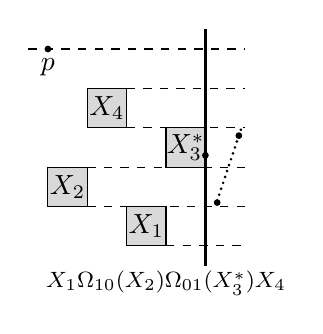
\begin{tikzpicture}[scale=0.5]
    % dashed lines
    \draw[dashed] (2,4) -- (5,4);
    \draw[dashed] (2,3) -- (5,3);
    \draw[dashed] (1,2) -- (5,2);
    \draw[dashed] (1,1) -- (5,1);
    \draw[dashed] (3,0) -- (5,0);
    \draw[dashed] (-0.5,5) -- (5,5); % p-line
%    \draw[dashed] (-2,9) -- (10,9); % q-line
    
    \filldraw[black] (0,5) circle (2pt) node[below]{$p$};
%    \filldraw[black] (-2,9) circle (2pt) node[above]{$q$};
    
    \draw[fill=gray!30] (1,3) rectangle (2,4) node[pos=0.5]{$X_4$};
    \draw[fill=gray!30] (3,2) rectangle (4,3) node[pos=0.5]{$X^*_3$};
    \draw[fill=gray!30] (0,1) rectangle (1,2) node[pos=0.5]{$X_2$};
    \draw[fill=gray!30] (2,0) rectangle (3,1) node[pos=0.5]{$X_1$};
    \draw[-, very thick] (4,-0.5) -- (4,5.5);
    \filldraw[black] (4,2.3) circle (2pt);

    \foreach \i in {1,...,13}
    {
      \filldraw[black] (4.25+0.05*\i,1+0.15*\i) circle (0.5pt);
    }
    \filldraw[black] (4.3,1.1) circle (2pt);
    \filldraw[black] (4.85,2.8) circle (2pt);
    \draw (3,-1.5) node[above]{\footnotesize $X_1\Omega_{10}(X_2)\Omega_{01}(X_3^*)X_4\Z$};
  \end{tikzpicture}\hfill
  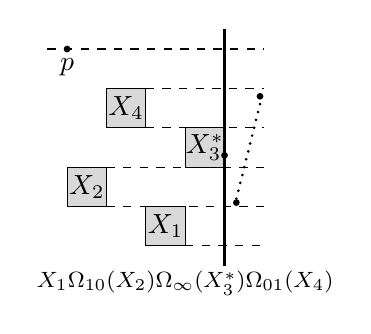
\begin{tikzpicture}[scale=0.5]
    % dashed lines
    \draw[dashed] (2,4) -- (5,4);
    \draw[dashed] (2,3) -- (5,3);
    \draw[dashed] (1,2) -- (5,2);
    \draw[dashed] (1,1) -- (5,1);
    \draw[dashed] (3,0) -- (5,0);
    \draw[dashed] (-0.5,5) -- (5,5); % p-line
%    \draw[dashed] (-2,9) -- (10,9); % q-line
    
    \filldraw[black] (0,5) circle (2pt) node[below]{$p$};
%    \filldraw[black] (-2,9) circle (2pt) node[above]{$q$};
    
    \draw[fill=gray!30] (1,3) rectangle (2,4) node[pos=0.5]{$X_4$};
    \draw[fill=gray!30] (3,2) rectangle (4,3) node[pos=0.5]{$X^*_3$};
    \draw[fill=gray!30] (0,1) rectangle (1,2) node[pos=0.5]{$X_2$};
    \draw[fill=gray!30] (2,0) rectangle (3,1) node[pos=0.5]{$X_1$};
    \draw[-, very thick] (4,-0.5) -- (4,5.5);
    \filldraw[black] (4,2.3) circle (2pt);

    \foreach \i in {1,...,14}
    {
      \filldraw[black] (4.25+0.05*\i,1+0.2*\i) circle (0.5pt);
    }
    \filldraw[black] (4.3,1.1) circle (2pt);
    \filldraw[black] (4.9,3.8) circle (2pt);
    \draw (3,-1.5) node[above]{\footnotesize $X_1\Omega_{10}(X_2)\Omega_\infty(X_3^*)\Omega_{01}(X_4)\Z$};
  \end{tikzpicture}\\ \ \\
  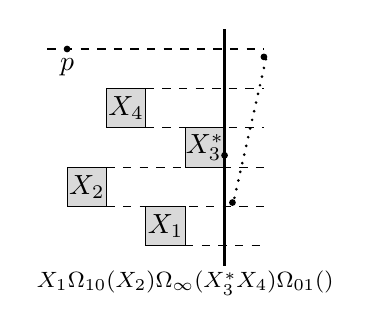
\begin{tikzpicture}[scale=0.5]
    % dashed lines
    \draw[dashed] (2,4) -- (5,4);
    \draw[dashed] (2,3) -- (5,3);
    \draw[dashed] (1,2) -- (5,2);
    \draw[dashed] (1,1) -- (5,1);
    \draw[dashed] (3,0) -- (5,0);
    \draw[dashed] (-0.5,5) -- (5,5); % p-line
%    \draw[dashed] (-2,9) -- (10,9); % q-line
    
    \filldraw[black] (0,5) circle (2pt) node[below]{$p$};
%    \filldraw[black] (-2,9) circle (2pt) node[above]{$q$};
    
    \draw[fill=gray!30] (1,3) rectangle (2,4) node[pos=0.5]{$X_4$};
    \draw[fill=gray!30] (3,2) rectangle (4,3) node[pos=0.5]{$X^*_3$};
    \draw[fill=gray!30] (0,1) rectangle (1,2) node[pos=0.5]{$X_2$};
    \draw[fill=gray!30] (2,0) rectangle (3,1) node[pos=0.5]{$X_1$};
    \draw[-, very thick] (4,-0.5) -- (4,5.5);
    \filldraw[black] (4,2.3) circle (2pt);

    \foreach \i in {1,...,17}
    {
      \filldraw[black] (4.2+0.05*\i,1+0.22*\i) circle (0.5pt);
    }
    \filldraw[black] (4.2,1.1) circle (2pt);
    \filldraw[black] (5,4.8) circle (2pt);
    \draw (3,-1.5) node[above]{\footnotesize $X_1\Omega_{10}(X_2)\Omega_\infty(X_3^*X_4)\Omega_{01}(\Z)$};
  \end{tikzpicture}
  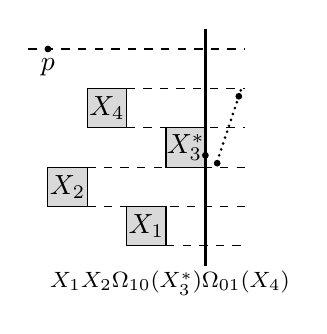
\begin{tikzpicture}[scale=0.5]
    % dashed lines
    \draw[dashed] (2,4) -- (5,4);
    \draw[dashed] (2,3) -- (5,3);
    \draw[dashed] (1,2) -- (5,2);
    \draw[dashed] (1,1) -- (5,1);
    \draw[dashed] (3,0) -- (5,0);
    \draw[dashed] (-0.5,5) -- (5,5); % p-line
%    \draw[dashed] (-2,9) -- (10,9); % q-line
    
    \filldraw[black] (0,5) circle (2pt) node[below]{$p$};
%    \filldraw[black] (-2,9) circle (2pt) node[above]{$q$};
    
    \draw[fill=gray!30] (1,3) rectangle (2,4) node[pos=0.5]{$X_4$};
    \draw[fill=gray!30] (3,2) rectangle (4,3) node[pos=0.5]{$X^*_3$};
    \draw[fill=gray!30] (0,1) rectangle (1,2) node[pos=0.5]{$X_2$};
    \draw[fill=gray!30] (2,0) rectangle (3,1) node[pos=0.5]{$X_1$};
    \draw[-, very thick] (4,-0.5) -- (4,5.5);
    \filldraw[black] (4,2.3) circle (2pt);

    \foreach \i in {1,...,13}
    {
      \filldraw[black] (4.25+0.05*\i,2+0.15*\i) circle (0.5pt);
    }
    \filldraw[black] (4.3,2.1) circle (2pt);
    \filldraw[black] (4.85,3.8) circle (2pt);
    \draw (3.1,-1.5) node[above]{\footnotesize $X_1X_2\Omega_{10}(X_3^*)\Omega_{01}(X_4)\Z$};
  \end{tikzpicture}\hfill
  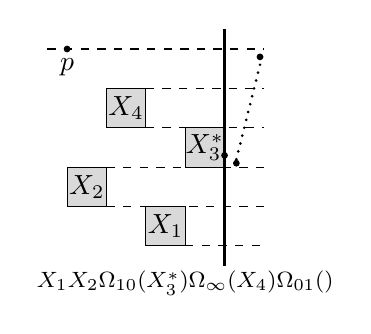
\begin{tikzpicture}[scale=0.5]
    % dashed lines
    \draw[dashed] (2,4) -- (5,4);
    \draw[dashed] (2,3) -- (5,3);
    \draw[dashed] (1,2) -- (5,2);
    \draw[dashed] (1,1) -- (5,1);
    \draw[dashed] (3,0) -- (5,0);
    \draw[dashed] (-0.5,5) -- (5,5); % p-line
%    \draw[dashed] (-2,9) -- (10,9); % q-line
    
    \filldraw[black] (0,5) circle (2pt) node[below]{$p$};
%    \filldraw[black] (-2,9) circle (2pt) node[above]{$q$};
    
    \draw[fill=gray!30] (1,3) rectangle (2,4) node[pos=0.5]{$X_4$};
    \draw[fill=gray!30] (3,2) rectangle (4,3) node[pos=0.5]{$X^*_3$};
    \draw[fill=gray!30] (0,1) rectangle (1,2) node[pos=0.5]{$X_2$};
    \draw[fill=gray!30] (2,0) rectangle (3,1) node[pos=0.5]{$X_1$};
    \draw[-, very thick] (4,-0.5) -- (4,5.5);
    \filldraw[black] (4,2.3) circle (2pt);

    \foreach \i in {1,...,14}
    {
      \filldraw[black] (4.25+0.05*\i,2+0.2*\i) circle (0.5pt);
    }
    \filldraw[black] (4.3,2.1) circle (2pt);
    \filldraw[black] (4.9,4.8) circle (2pt);
    \draw (3,-1.5) node[above]{\footnotesize $X_1X_2\Omega_{10}(X_3^*)\Omega_\infty(X_4)\Omega_{01}(\Z)$};
  \end{tikzpicture}\\ \ \\
\caption{We apply $\Omega_{11}$ to $\T = X_1X_2X_3^*X_4p$. Inflation $2413[X_2,X_4,X_1,X_3]$ represents $X_1X_2X_3^*X_4$. Lowest and top-most points on the RHS are bold (distinguished under $\Omega_{11}$). Lowest point on RHS is below right-most point on LHS.}
\label{fig:iterjuxt_omega11action}
\end{figure}

\newpage
\section{Main results}
\label{sec:iterjuxt_main}

Just briefly in this first paragraph we use context-free to refer to ``context-free admitting a combinatorial specification tracking the right-most point''. This section presents general results that we are able to obtain with the tools set up in Section~\ref{sec:iterjuxt_intro}. First, we prove that a juxtaposition of a non-empty context-free cell with a non-empty monotone increasing cell is context free. This invariant is stated as Lemma~\ref{lem:induction_step} and we need it for the proof of the key result, Proposition~\ref{prop:onesidedjuxt}. In Proposition~\ref{prop:onesidedjuxt}, we state that appending monotone increasing classes on the right side of a context-free permutation class does not change the character of the original combinatorial specification and hence the generating function of the obtained juxtaposition class is algebraic. Next we prove that by left-right flips and up-down flips, we can rephrase appending a decreasing monotone permutation class into appending an increasing monotone permutation class, and we can do so on either side of $\C$ (left or right). This is established in Propositions~\ref{prop:decrappend} and~\ref{prop:leftappend}. Therefore, it turns out that appending a monotone class (increasing or decreasing) on either side of a context-free permutation class preserves the character of the combinatorial specification and hence the character of the generating function of such a class. We use induction to prove that after finitely many such juxtapositions, the resulting class is still context-free and is enumerated by an algebraic generating function. This is our main result and is stated as Theorem~\ref{thm:iterjuxt_main}. In addition to this general setting, we show in a Corollary~\ref{cor:finmanysimples} that the same holds for all permutation classes with finitely many simple permutations. These form a large special case.

Let us now state the key lemma expressing the ``context-freeness invariant'' with care.


\begin{lemma}
  \label{lem:induction_step}
  Let $\C$ be a context-free permutation class and let $\rS$ be its combinatorial specification which tracks the rightmost point of $\C$ by vertical position (value). Let $\M$ be a monotone increasing permutation class. Consider a class $\C'$ of permutations $\pi$ which admit our usual leftmost gridding as $\pi=\pi_1|\pi_2$ where $\pi_1\in \C$ and $\pi_2\in \M$ and neither $\pi_1$ nor $\pi_2$ is empty. Then $\C'$ is context-free and admits a combinatorial specification $\rS'$ that tracks the rightmost point by vertical position (value).
\end{lemma}
\begin{proof}
In the language of $\Omega$ operators, expressing $\C'$ requires installing a phantom point $p$ above $\C$ to construct $\barCstar$. Furthermore, we will express $\C'\Z$ instead of $\C'$, since removing the phantom point from each permutation in $\C'\Z$ is simply a matter of later removing that trailing $\Z$ from every term (product) $\T$ in its combinatorial specification. Notice that every term $\T$ indeed has such a $\Z$ at the end of it as every term has a phantom point on top. This means that if $\C'\Z$ has a context-free specification that tracks the rightmost point by value, then so does $\C'$. Therefore, the expression for $\C'\Z$ is the following one.
\begin{align}
  \C'\Z = \Omega_1(\barCstar) + \Omega_{11}(\barCstar).
  \label{eq:induction_step_expression}
\end{align}
Notice that as defined, $\C'\Z$ is merely a combinatorial class (as opposed to a permutation class) because it does not contain $\EE + \M$. Given that $\C'\Z$ is simply a building block in claims about permutation classes, we do not need $\C'\Z$ itself to be a permutation class. It now remains to show two things
\begin{enumerate}
\item $\Omega_1(\barCstar) + \Omega_{11}(\barCstar)$ indeed represents $\C'\Z$.
\item $\Omega_1(\barCstar)$ and $\Omega_{11}(\barCstar)$ admit context-free combinatorial specifications that track the rightmost points.
\end{enumerate}
If 1. is true, then we simply know that we are proving the right thing. If also 2. is true, then $\Omega_1(\barCstar) + \Omega_{11}(\barCstar)$ also admits a context-free combinatorial specification that tracks the rightmost point and by 1. we have indeed shown that the conclusion of Lemma~\ref{lem:induction_step} holds.

Let us begin by proving 1. This follows from the definitions of $\Omega_1$ and $\Omega_{11}$. We only briefly describe how as it is straightforward yet tedious. One has to accept that $\Omega_1$ represents a cell with a single point juxtaposed on the right of its argument so that this point is always below the rightmost point of the left cell (to ensure the leftmost possible gridding). We recall the definition of $\Omega_1$.
\begin{align*}
    \Omega_1(\Z) &= \Z^*\Z\\
    \Omega_1(\Z^*) &= \Z^*\Z\\
  \Omega_1(\T_h) &=
                      \begin{cases}
                        \Omega_1(X_1^*)\Omega_0(X_2\cdots X_m) \quad &\text{if $k = 1$}\\
                        \Omega_1(X_1)\Omega_0(X_2\cdots X_m) + \Omega_0(X_1)\Omega_1(X_2\cdots X_m),\quad &\text{if $k>1$.}
                      \end{cases}
\end{align*}
The base cases clearly do juxtapose a point on the RHS below the point on the LHS. See Figure~\ref{fig:omega_1} and recall that reading the Cartesian product left-to-right reflects the bottom-to-top order in the permutation. As for the recursive step, notice that if the rightmost point is in the bottom-most term of the product, then we do not apply $\Omega_1$ above it at all (and so the leftmost point on the RHS is not above the rightmost point on the LHS). Operator $\Omega_0$ is applied to the rest of the terms in the product, meaning that there is nothing on the RHS next to those terms. If the bottom-most term of the product does not contain the rightmost point, then there are two options. Either the single point on the RHS is next to this term or it is not. These are the two expressions on the second line of the recursive step. Notice that second term involves a recursion on the tail of the product which is strictly shorter in length than $\T_h$, so the procedure terminates. And therefore, $\Omega_1$ indeed represents a juxtaposition of two non-empty cells as desired, provided that its argument is non-empty (which we make sure it is). To show that $\Omega_{11}$ correctly expresses the juxtaposition we want is slightly more complicated. The definition of $\Omega_{11}$ depends on the definitions of $\Omega_{10}, \Omega_{01}, \Omega_\infty$ and requires a more tedious verification which we do not do here. However, in Figure~\ref{fig:iterjuxt_omega11action} we demonstrate the definition of $\Omega_{11}$ on a simple $\T_h$ to make it easier to work through the definition. We conclude that point 1. is valid.

To show that 2. holds, we need to revisit the definitions of $\Omega_1$ and $\Omega_{11}$ again. Notice that items of the form $\Omega_i(X)$ (for $X\in \V$) will need to be added to $\V$. We work our way through the definition $\Omega_1$ and leave $\Omega_{11}$ to the reader as it is analogous but significantly longer. The goal is to show that $\Omega_1$ preserves the context-freeness of the combinatorial specification of its input and correctly replaces the right-most point in the input with the new right-most point (the single point on the RHS). Looking at the definition above, $\Omega_1$ does two things. One, it replaces $\Z$ with $\Zstar\Z$ or $\Zstar$ with $\Zstar\Z$. Two, it splits a product $\T_h$ into two products: $\Omega_1(X_1)\Omega_0(X_2\cdots X_m)$ and $\Omega_0(X_1)\Omega_1(X_2\cdots X_m)$. Each of these products has $\Omega_1$ applied to a smaller expression than $\T_h$ and by induction those are of the correct form. The rest of each of the two products has $\Omega_0$ applied to it which does not change that part of the expression. Therefore, given that $\Omega_1$ is linear over $+$, it indeed preserves the context-freeness of the combinatorial specification of its input. We argued that the rightmost point gets tracked correctly in 1. This concludes our task for $\Omega_1$. Similarly, one can verify that $\Omega_{11}$ produces a context-free output that tracks the rightmost point, provided the input is of this form.

As shown before, 1. together with 2. imply the statement of Lemma~\ref{lem:induction_step}. 
\end{proof}

\begin{proposition}
  \label{prop:onesidedjuxt}
  Let $\C$ be a context-free permutation class and $\rS$ its combinatorial specification which tracks the rightmost point of $\C$ by vertical position (value). Let $\M_1,\ldots,\M_k$ be a sequence of monotone increasing permutation classes. Then $\C|\M_1|\ldots|\M_k$ admits a context-free combinatorial specification which tracks the rightmost point by value. Consequently, $\C|\M_1|\ldots|\M_k$ admits an algebraic generating function.
\end{proposition}
\begin{proof}
  We prove by induction that for every $k \geq 1$, the class $\C|\M_1|\ldots|M_k$ admits a context-free combinatorial specification which tracks the rightmost point by value. It then follows that there also exists a context-free combinatorial specification of such a class, simply by dropping ${}^*$ and ${}^\circ$ decorations. Consequently, it follows by Theorem~\ref{thm:chomsky} that $\C|\M_1|\ldots|\M_k$ admits a generating function that is algebraic.

  First, notice that we can rewrite the original juxtaposition as follows to obtain disjoint terms and every cell in each term non-empty.
\begin{align}
  \C|\M_1|\ldots|\M_k &= \EE + \M'_k + \ldots + \M'_1|\ldots|\M'_k  + \C'|\M'_1|\ldots|\M'_k,
\label{eq:rewritten}
\end{align}
 where, for the moment, $\M'$ and $\C'$ denote the non-empty versions of the respective classes. To see where each term comes from, recall that we grid greedily from the right. So if all $k$ cells are empty, then the cell with $\C$ must also be empty and this is represented by $\EE$. If there is one non-empty cell, then it must be $\M_k$ --- again thanks to the greedy gridding from the right. We continue this way and obtain exactly~\eqref{eq:rewritten}. Furthermore, since all $\M_i$ are identical, it follows that $\M_1'|\ldots|\M_{k-1}' = \M_2'|\ldots|\M_{k}'$. We will use this during induction.

\noindent \textbf{Base case:}\\
\noindent If $k = 1$, then~\eqref{eq:rewritten} has the following form.
\begin{align}
  \C|\M_1 &= \EE + \M'_1 + \C'|\M'_1
  \label{eq:basecase}
\end{align}
Clearly, $\M_1'$ is context-free and admits a combinatorial specification which tracks the rightmost point by value (we saw this in Section~\ref{sec:iterjuxt_intro} as $\Mstar$). By Lemma~\ref{lem:induction_step}, $\C'|\M_1'$ is also context-free and admits a combinatorial specification which tracks the rightmost point by value. Therefore, $\C|\M_1$ is context-free and admits the right combinatorial specification --- we are done.

\noindent \textbf{Induction step:}\\
\noindent For any $k$ greater than $1$, let $\C_0' = \C'|\M'_1|\ldots|\M'_{k-1}$. By induction assumption, $\C_0'$ is context-free and admits a combinatorial specification that tracks the rightmost point by value. This is the case as $\C_0 = \C|\M_1|\ldots|\M_{k-1}$ is all that by induction assumption and $\C_0'$ is one term of an expression like~\eqref{eq:rewritten} for $\C_0$. Therefore, we need to show that $\C_0'|\M_k'$ is context-free and admits the right combinatorial specification. But $\C_0'$ and $\M_k'$ meet the conditions of Lemma~\ref{lem:induction_step} and hence the claim follows. The only term in~\eqref{eq:rewritten} which does not fall within the induction assumption in an obvious way is $\M_2'|\ldots|\M_k'$. There was no $1\times k-1$ row of non-empty monotone cells in an expression like~\eqref{eq:rewritten} for $\C|\M_1|\ldots|\M_{k-1}$. On the other hand, $\M_2$ is a context-free class that admits a combinatorial specification which tracks the rightmost point by value. Therefore, let $\C_\M = \M_2$, and we get $\M_2'|\ldots|\M_k' = \C_\M'|\M_3'|\ldots|\M_k'$. Now, this juxtaposition of non-empty cells does fall under the induction assumption and we are done. Every term in~\eqref{eq:rewritten} is context-free and admits a combinatorial specification which tracks the rightmost point by value. Therefore, $\C|\M_1|\ldots|\M_k$ is such a context-free class and the Proposition~\ref{prop:onesidedjuxt} follows.
\end{proof}

The major message in Lemma~\ref{lem:induction_step} is that juxtaposing a monotone increasing class on the right of a context-free class does not qualitatively affect the context-free class that we started with. This turns out to be a key invariant as it lends itself to repeated juxtapositions. That is the other crucial message and we introduced it in Proposition~\ref{prop:onesidedjuxt} as ``repeated juxtaposing is allowed'' for monotone increasing classes on the right side of a context-free class. These two building blocks are going to be used as black boxes when we generalise the increasing monotone classes to any monotone classes and allow the juxtapositions on both sides of the context-free class. 


\subsection{Extension to decreasing classes and both sides}
\label{sec:extensions}

As advertised, this subsection transforms more general juxtapositions into a form that Lemma~\ref{lem:induction_step} and Proposition~\ref{prop:onesidedjuxt} can deal with. The culmination is Theorem~\ref{thm:iterjuxt_main} which concludes that finitely many juxtapositions of any monotone classes on either side of a context-free class form a context-free class, which thereby admits an algebraic generating function.

We begin by proving that it is possible to append decreasing monotone classes on the right-hand side of a context-free class.
\begin{proposition}
  \label{prop:decrappend}
  Let $\DD$ be a monotone decreasing permutation class and $\C$ a context-free permutation class that admits a combinatorial specification which tracks the right-most point by value. Then $\C|\DD$ admits a combinatorial specification which tracks the rightmost point by value.
\end{proposition}
\begin{proof}
We reduce the juxtaposition $\C|\DD$ to a juxtaposition of the form $\reflectbox{\rotatebox[origin=c]{180}{\C}}|\M$ (an upside-down $\C|\DD$). However, there are several details that require attention. For instance, in a juxtaposition $\C|\M$, a point $x$ on the LHS is associated with a sequence on the RHS that falls into the gap immediately below $x$, see Figure~\ref{fig:xregion}. If we want this to be the case for the juxtaposition $\reflectbox{\rotatebox[origin=c]{180}{\C}}|\M$, we must start by associating points on the RHS of $\C|\DD$ \emph{above} the points on the LHS. Similarly, If we want an upper phantom point $p$ to be above and to the left of $\reflectbox{\rotatebox[origin=c]{180}{\C}}|\M$, we must start with a lower phantom point $q$ as in $q \oplus \C|\DD$. Given this set-up, we write $\C|\DD$ as a sum of disjoint terms. 
\begin{align}
  \C|\DD = \EE + \DD' + \C'|\DD',
\label{eq:decrease_objective}
\end{align}
where $\C'$ and $\DD'$ are non-empty versions of $\C$ and $\DD'$, respectively.

\begin{figure}[!ht]
  \centering
  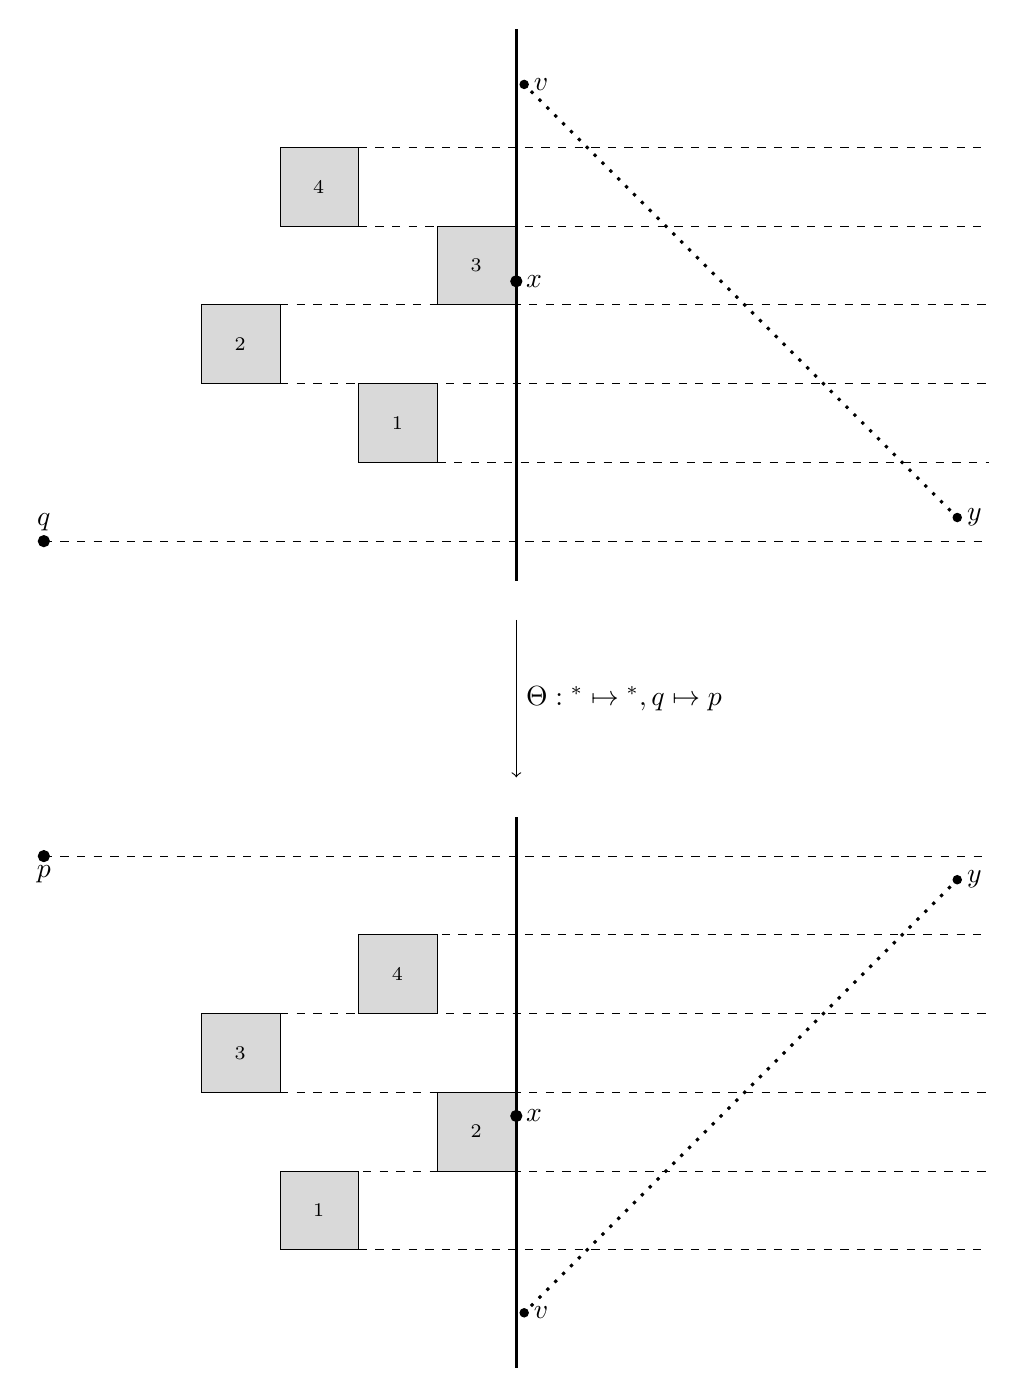
\begin{tikzpicture}
    \draw[dashed] (2,14) -- (10,14);
    \draw[dashed] (2,13) -- (10,13);
    \draw[dashed] (1,12) -- (10,12);
    \draw[dashed] (1,11) -- (10,11);
    \draw[dashed] (3,10) -- (10,10);
%    \draw[dashed] (-1,15) -- (10,15); % p-line
    \draw[dashed] (-2,9) -- (10,9); % q-line
    
%    \filldraw[black] (-1,15) circle (2pt) node[below]{$p$};
    \filldraw[black] (-2,9) circle (2pt) node[above]{$q$};
    
    \draw[fill=gray!30] (1,13) rectangle (2,14) node[pos=0.5]{$\C_4$};
    \draw[fill=gray!30] (3,12) rectangle (4,13) node[pos=0.5]{$\Cstar_3$};
    \draw[fill=gray!30] (0,11) rectangle (1,12) node[pos=0.5]{$\C_2$};
    \draw[fill=gray!30] (2,10) rectangle (3,11) node[pos=0.5]{$\C_1$};
    \draw[-, very thick] (4,8.5) -- (4,15.5);
    \filldraw[black] (4,12.3) circle (2pt) node[right]{$x$};

    \foreach \i in {1,...,55}
    {
      \filldraw[black] (4.1+0.1*\i,14.8-0.1*\i) circle (0.5pt);
    }
    \filldraw[black] (4.1,14.8) circle (1.5pt) node[right]{$v$};
    \filldraw[black] (9.6,9.3) circle (1.5pt) node[right]{$y$};

    \draw[->] (4,8)--(4,6);
    \filldraw[black] (4,7) circle (0pt) node[right]{$\Theta: {}^* \mapsto {}^*, q \mapsto p$};

    \draw[dashed] (2,4) -- (10,4);
    \draw[dashed] (1,3) -- (10,3);
    \draw[dashed] (1,2) -- (10,2);
    \draw[dashed] (1,1) -- (10,1);
    \draw[dashed] (2,0) -- (10,0);
    \draw[dashed] (-2,5) -- (10,5); % p-line
 %   \draw[dashed] (-1,-1) -- (10,-1); % q-line
    
    \filldraw[black] (-2,5) circle (2pt) node[below]{$p$};
%    \filldraw[black] (-1,-1) circle (2pt) node[above]{$p$};
    
    \filldraw[fill=gray!30] (2,3) rectangle (3,4) node[pos=0.5]{$\HH_4$};
    \draw[fill=gray!30] (0,2) rectangle (1,3) node[pos=0.5]{$\HH_3$};
    \draw[fill=gray!30] (3,1) rectangle (4,2) node[pos=0.5]{$\HHstar_2$};
    \draw[fill=gray!30] (1,0) rectangle (2,1) node[pos=0.5]{$\HH_1$};
    \draw[-, very thick] (4,-1.5) -- (4,5.5);
    \filldraw[black] (4,1.7) circle (2pt) node[right]{$x$};

    \foreach \i in {1,...,55}
    {
      \filldraw[black] (4.1+0.1*\i,-0.8+0.1*\i) circle (0.5pt);
    }
    \filldraw[black] (4.1,-0.8) circle (1.5pt) node[right]{$v$};
    \filldraw[black] (9.6,4.7) circle (1.5pt) node[right]{$y$};
  \end{tikzpicture}
\caption{Appending a monotone decreasing class to $\C$ amounts to appending a monotone increasing class to $\C$ upside-down. In the notation of the figure, $\C_1= \HH_4$, $\C_2 =\HH_3$, $\Cstar_3 = \HHstar_2$, and $\C_4 = \HH_1$. Before the flip one needs to associate decorations with gaps above LHS points, not below LHS points. Additionally, the lower phantom point which is transformed to the upper phantom point by the upside-down flip.}
\label{fig:horizontal_flip}
\end{figure}

We transform $q\oplus\C^*|\DD$ into $p\ominus\reflectbox{\rotatebox[origin=c]{180}{\C}}^*|\M$ by a flip along the horizontal axis --- otherwise known as complementation. We call the operator that does this job $\Theta$. The rightmost point stays right-most after the flip, i.e. $\Theta({}^*) = {}^*$. The phantom point $q$ assumes the usual position of the phantom point $p$, i.e. $\Theta(q) = p$, a mere renaming. The points on the RHS now appear below the ones on the LHS that they are associated with. It goes without saying that a bottom-to-top specification can be simply reversed into a top-to-bottom specification in order to facilitate the upside-down flip. The entire situation is analogous to the one in Lemma~\ref{lem:induction_step}. The only term we need to worry about is when both $\C$ and $\DD$ are non-empty. Writing the juxtaposition of two non-empty cells in terms of $\Omega$ operators gives the following expression.
$$\C'|\DD' = \Theta^{-1}(\Omega_1(\Theta(q\oplus \Cstar))) + \Theta^{-1}(\Omega_{11}(\Theta(q \oplus \Cstar))).$$ 
In other words, we can use all the infrastructure that is in place for monotone increasing classes to append monotone decreasing classes. Since $\Theta$ is bijective, we transform the decreasing setting into increasing, apply the operators we need to apply, and then bring the situation back by $\Theta^{-1}$. Figure~\ref{fig:horizontal_flip} gives an instance of the upside-down flip transformation.
\end{proof}

\begin{proposition}
  \label{prop:leftappend}
Let $\DD$ be a monotone decreasing permutation class and $\C$ a context-free permutation class that admits a combinatorial specification which tracks the leftmost point. Then $\DD|\C$ is context-free and admits a combinatorial specification which tracks the leftmost.
\end{proposition}
\begin{figure}[!ht]
  \centering
  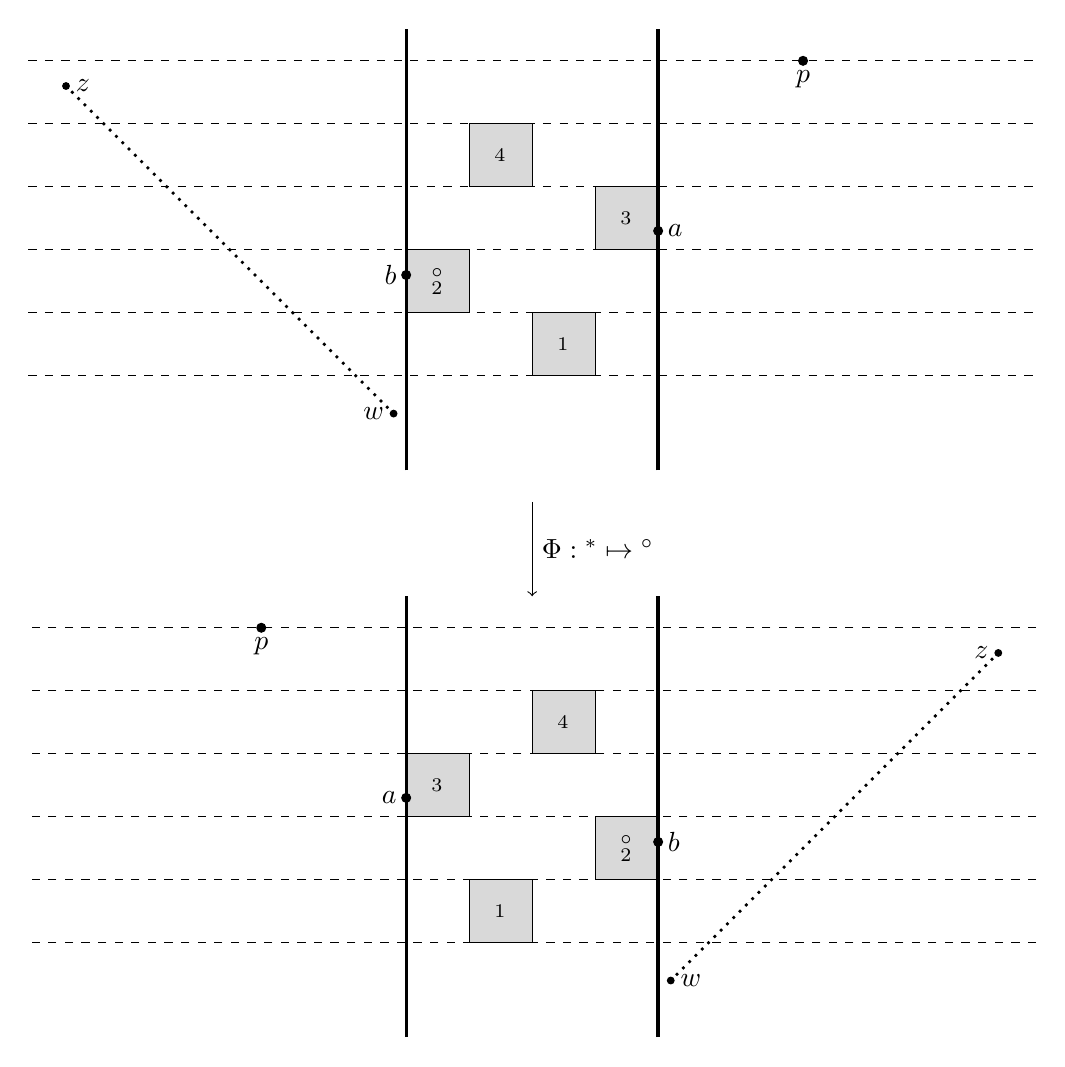
\begin{tikzpicture}[scale=0.8]
    \begin{scope}[xshift=-0.5cm]
    \draw[dashed] (-6,14) -- (10,14);
    \draw[dashed] (-6,13) -- (10,13);
    \draw[dashed] (-6,12) -- (10,12);
    \draw[dashed] (-6,11) -- (10,11);
    \draw[dashed] (-6,10) -- (10,10);
    \draw[dashed] (-6,15) -- (10,15); % p-line
%    \draw[dashed] (-6,9) -- (10,9); % q-line
    
    \filldraw[black] (6.3,15) circle (2pt) node[below]{$p$};
%    \filldraw[black] (-2,9) circle (2pt) node[above]{$q$};
    
    \draw[fill=gray!30] (1,13) rectangle (2,14) node[pos=0.5]{$\C_4$};
    \draw[fill=gray!30] (3,12) rectangle (4,13) node[pos=0.5]{$\Cstar_3$};
    \draw[fill=gray!30] (0,11) rectangle (1,12) node[pos=0.5]{$\C_2^\circ$};
    \draw[fill=gray!30] (2,10) rectangle (3,11) node[pos=0.5]{$\C_1$};
    \draw[-, very thick] (4,8.5) -- (4,15.5);
    \draw[-, very thick] (0,8.5) -- (0,15.5);
    \filldraw[black] (4,12.3) circle (2pt) node[right]{$a$};
    \filldraw[black] (0,11.6) circle (2pt) node[left]{$b$};
    
    % RHS
    % \foreach \i in {1,...,55}
    % {
    %   \filldraw[black] (4.1+0.1*\i,14.8-0.1*\i) circle (0.5pt);
    % }
    % \filldraw[black] (4.1,14.8) circle (1.5pt) node[right]{$u$};
    % \filldraw[black] (9.6,9.3) circle (1.5pt) node[right]{$v$};

    % LHS
    \foreach \i in {1,...,53}
    {
      \filldraw[black] (-5.5+0.1*\i,14.7-0.1*\i) circle (0.5pt);
    }
    \filldraw[black] (-0.2,9.4) circle (1.5pt) node[left]{$w$};
    \filldraw[black] (-5.4,14.6) circle (1.5pt) node[right]{$z$};
    \end{scope}

    \draw[->] (1.5,8)--(1.5,6.5);
    \filldraw[black] (1.5,7.25) circle (0pt) node[right]{$\Phi: {}^*\mapsto{}^\circ$};


    %==================== reflection ======================
    \begin{scope}[xscale=-1, xshift=-3.5cm, yshift=-9cm]
    \draw[dashed] (-6,14) -- (10,14);
    \draw[dashed] (-6,13) -- (10,13);
    \draw[dashed] (-6,12) -- (10,12);
    \draw[dashed] (-6,11) -- (10,11);
    \draw[dashed] (-6,10) -- (10,10);
    \draw[dashed] (-6,15) -- (10,15); % p-line
%    \draw[dashed] (-6,9) -- (10,9); % q-line
    
    \filldraw[black] (6.3,15) circle (2pt) node[below]{$p$};
%    \filldraw[black] (-2,9) circle (2pt) node[above]{$q$};
    
    \draw[fill=gray!30] (1,13) rectangle (2,14) node[pos=0.5]{$\C_4$};
    \draw[fill=gray!30] (3,12) rectangle (4,13) node[pos=0.5]{$\Cstar_3$};
    \draw[fill=gray!30] (0,11) rectangle (1,12) node[pos=0.5]{$\C_2^\circ$};
    \draw[fill=gray!30] (2,10) rectangle (3,11) node[pos=0.5]{$\C_1$};
    \draw[-, very thick] (4,8.5) -- (4,15.5);
    \draw[-, very thick] (0,8.5) -- (0,15.5);
    \filldraw[black] (4,12.3) circle (2pt) node[left]{$a$};
    \filldraw[black] (0,11.6) circle (2pt) node[right]{$b$};
    
    % RHS
    % \foreach \i in {1,...,55}
    % {
    %   \filldraw[black] (4.1+0.1*\i,14.8-0.1*\i) circle (0.5pt);
    % }
    % \filldraw[black] (4.1,14.8) circle (1.5pt) node[right]{$u$};
    % \filldraw[black] (9.6,9.3) circle (1.5pt) node[right]{$v$};

    % LHS
    \foreach \i in {1,...,53}
    {
      \filldraw[black] (-5.5+0.1*\i,14.7-0.1*\i) circle (0.5pt);
    }
    \filldraw[black] (-0.2,9.4) circle (1.5pt) node[right]{$w$};
    \filldraw[black] (-5.4,14.6) circle (1.5pt) node[left]{$z$};
    \end{scope}
  \end{tikzpicture}
  \caption{Left-to-right flip swaps starred and circled points (or classes) and causes the monotone class to change from decreasing to increasing or vice versa. We also begin with a point $p$ which is not a phantom point as it is to the right of $\C$. It becomes a phantom point after $\Phi$ is applied to the set-up. The bottom picture is the arrangement representing the action of $\Omega$ operators.}
  \label{fig:phi_flip}
\end{figure}
\begin{proof}
Similar to the upside-down flip in Proposition~\ref{prop:decrappend}, the proof proceeds by transformation of $\C$ via a left-to-right flip $\Phi$, then applying $\Omega$ operators, and undoing the flip. In the process, we need to make sure that the left-most and the rightmost points are treated correctly, and that the phantom points work as expected. For this purpose, we need to keep track of the left-most point of $\C$. First, we require that the combinatorial specification of $\C$ tracks the leftmost point of $\C$. Recall that we denote the objects containing the leftmost point by $\C^\circ$ or $\Z^\circ$. As before, enumerating $\DD|\C$ amounts to enumerating the juxtaposition of two non-empty cells where the one on the left-hand side is $\DD'$ and the one on the right-hand side is $\C'$. If $\Phi$ is the left-to-right flip operator, then enumerating $\DD|\C$ is the same as enumerating $\reflectbox{\C}|\M$, where $\M$ stands for monotone increasing class, if we remember to keep track of the details (critical points). In particular, $\Phi(\Z^\circ) = \Phi(\Z^*)$ and $\Phi(\Z^*) = \Phi(\Z^\circ)$. In contrast to the upside-down flip operator $\Theta$, we begin with appending an invalid phantom point to $\C$, which becomes valid after the flip, and is removed afterwards when $\Phi$ is undone. Please refer to Figure~\ref{fig:phi_flip} for a visual guide. 
$$\DD'|\C' = \Phi^{-1}(\Omega_1(\Phi(\C^\circ\oplus p))) + \Phi^{-1}(\Omega_{11}(\Phi(\C^\circ\oplus p))).$$
It is clear that after the transformation by $\Phi$, the arrangement is suitable for application of $\Omega$ operators. The correctness follows from Lemma~\ref{lem:induction_step} and Proposition~\ref{prop:onesidedjuxt}. Therefore, $\DD|\C$ admits a combinatorial specification which tracks the rightmost point.
\end{proof}
Notice that by Proposition~\ref{prop:decrappend} and Proposition~\ref{prop:leftappend}, appending increasing classes on the left-hand side also becomes possible. We wrap up our efforts in the following theorem.


\begin{theorem}
  \label{thm:iterjuxt_main}
  Let $\C$ be a context-free permutation class that admits a combinatorial specification which tracks both the right-most and the left-most points. Let $\M_1,\ldots,\M_{k+\ell}$ be a sequence of monotone, increasing or decreasing, permutation classes. Then $\M_1|\ldots|\M_k|\C|\M_{k+1}|\ldots|\M_{k+\ell}$ is a context-free permutation class that admits an algebraic generating function.
\end{theorem}
\begin{proof}
  Once we decide which gridding (from the left side or from the right side) gets priority, the claim follows by repeated applications of Proposition~\ref{prop:onesidedjuxt}, Proposition~\ref{prop:decrappend}, and Proposition~\ref{prop:leftappend}. Recall that the $\Omega$ operators only use the right-most point and ignore the presence of the left-most point (not deleting the circle, simply leaving it unchanged). Having both decorations (${}^*$ and ${}^\circ$) present in $\C$ at the same time does not negatively affect nor gets negatively affected by $\Omega$ operators.

  In short, Lemma~\ref{lem:induction_step} together with Proposition~\ref{prop:onesidedjuxt} guarantee that whatever we start with before the next juxtaposition is context-free and tracks the desired points correctly. Additionally, Proposition~\ref{prop:onesidedjuxt} also deals with the case when we append an increasing class on the right. The remaining cases are covered by first manipulating the situation via Proposition~\ref{prop:decrappend} and Proposition~\ref{prop:leftappend} into the arrangement when Proposition~\ref{prop:onesidedjuxt} applies again. Therefore, juxtaposing finitely many monotone classes on both sides of a context-free $\C$ leads to just another context-free class. Therefore, Theorem~\ref{thm:chomsky} then implies that the generating function of the resulting class is in fact algebraic.
\end{proof}

\begin{corollary}
 Let $\C$ be a context-free permutation class with finitely many simple permutations and let $\M_1,\ldots,\M_{k+\ell}$ be as in Theorem~\ref{thm:iterjuxt_main}. Then
 $$\M_1|\ldots|\M_k|\C|\M_{k+1}|\ldots|\M_{k+\ell}$$
 is a context-free permutation class which admits a generating function that is an algebraic function.
\label{cor:finmanysimples}
\end{corollary}
\begin{proof}
  We show that every context-free permutation class with finitely many simple permutations admits a combinatorial specification that tracks the right-most and left-most points. The claim then follows from Theorem~\ref{thm:iterjuxt_main}.

  If $\Si(\C)$ is the set of simple permutations in $\C$, we say that a vector $(\C_1,\ldots,\C_{|\sigma|})$ is admissible, if $\sigma \in \Si(\C)$ and $\sigma[\alpha_1,\ldots,\alpha_{|\sigma|}]$ is in $\C$ for all choices of $\alpha_i\in\C_i$. In case of $12$ or $21$, we insist that $\C_1$ in an admissible vector $(\C_1,\C_2)$ is always sum-indecomposable or skew-indecomposable, respectively. For convenience, we temporarily violate the customary notation about inflations. We use $\C_i$ to denote the $i$-th class from the bottom in the inflation of $\sigma$, i.e. $\sigma[\C_1,\ldots,\C_i,\ldots,\C_{|\sigma|}]$ means that the bottom-most point in $\sigma$ is inflated by $\C_1$, the point immediately above it in $\sigma$ is inflated by $\C_2$, and so on. In other words, we list the inflation by value instead of by position. Additionally, assume that the point with value $k_\sigma$ in $\sigma$ is the rightmost point of $\sigma$ and the point with value $\ell_\sigma$ is the left-most point of $\sigma$. Furthermore, we use a variable $X$ to stand for a class from $\{\C_1,\ldots,\C_r\}$. We now give the combinatorial specification template that every context-free class $\C$ with finitely many simples fits into. We only define the classes with both the left-most and the right-most points tracked. However, the combinatorial specification needs definitions of starred, circled, starles and circleless classes as well. Their definitions are analogous and take up a lot of space. We skip them.

  \begin{align}
    \begin{aligned}
    \C_1^{\circ*} &= \Z + \sum_{\substack{\text{admissible}\\(X_1,X_2)}}12[X_1^\circ,X_2^*] + \sum_{\substack{\text{admissible}\\(X_1,X_2)}}21[X_1^*,X_2^\circ] +\\
                   &+ \sum_{\sigma \in \Si(\C)}\sum_{\substack{\text{admissible}\\(\C_1,\ldots,\Cstar_k,\ldots,\C_\ell^\circ,\ldots,\C_{|\sigma|})}}\sigma[\C_1,\ldots,\Cstar_k,\ldots,\C_\ell^\circ,\ldots,\C_{|\sigma|}]\\
                   &\vdots\\
    \C_r^{\circ*} &= \Z + \sum_{\substack{\text{admissible}\\(X_1,X_2)}}12[X_1^\circ,X_2^*] + \sum_{\substack{\text{admissible}\\(X_1,X_2)}}21[X_1^*,X_2^\circ] +\\
                  &+ \sum_{\sigma \in \Si(\C)}\sum_{\substack{\text{admissible}\\(\C_1,\ldots,\Cstar_k,\ldots,\C_\ell^\circ,\ldots,\C_{|\sigma|})}}\sigma[\C_1,\ldots,\Cstar_k,\ldots,\C_\ell^\circ,\ldots,\C_{|\sigma|}]\\
                \end{aligned}
    \label{eq:proofcombspec}
  \end{align}
This completes the proof.
\end{proof}

Section~\ref{sec:example_sepav21} gives an example of a small non-trivial class with finitely many simple permutations (no simple permutations) --- the class of separable permutations, or $\S$. We know $\Si(\S) = \emptyset$ and therefore, the last terms on the RHS in~\eqref{eq:proofcombspec} vanishes. We enumerate exactly the juxtaposition of the class of separable permutations with the class of monotone increasing permutations. 

Notice that Corollary~\ref{cor:finmanysimples} is strictly weaker than Theorem~\ref{thm:iterjuxt_main}. For instance, $\Av(321)$ is a class with infinitely many simple permutations. Indeed, $2413$, $246135$, $24681357$, $\ldots$ are all $321$-avoiders and all of them are simple. Yet $\Av(321)$ admits a combinatorial specification required by Theorem~\ref{thm:iterjuxt_main}. We show this in Section~\ref{sec:example_Av321Av21} where we juxtapose it with a monotone increasing class and enumerate this juxtaposition exactly using methods developed in Section~\ref{sec:iterjuxt_intro}.

In Section~\ref{sec:example_mmm}, we enumerate exactly a repeated juxtaposition of the form $\C|\M|\M$ where $\C = \M$ and $\M$ is a monotone increasing class. 

\section{Applications to exact enumeration}
\subsection{Example: $\Av(321|21)$}
\label{sec:example_Av321Av21}

In Chapter~\ref{chap:catalanjuxt} we dealt with the juxtaposition of a Catalan class with a monotone class by enumerating all such juxtapositions. Here, we re-enumerate one of these cases, which also serves to illustrate that the method applies to classes other than those with finitely many simples. This demonstrates the gap between Corollary~\ref{cor:finmanysimples} and Theorem~\ref{thm:iterjuxt_main}.

We represent permutations in $\Av(321)$ by Dyck paths below the diagonal, starting in the bottom left corner and going to the top right corner of the grid. An exact definition of Dyck path can be found in Section~\ref{sec:catalanjuxt_defs}, including Figure~\ref{fig:dyckexample}. Also, below we replicate Figure~\ref{fig:bij321dyck} that demonstrates how we associate permutations from $\Av(321)$ with Dyck paths.

\begin{figure}[!ht]
\begin{center}
\begin{tikzpicture}[scale=0.2]
\dyck{0,0}{9}{black}{0,0,0,1,1,0,0,1,0,0,1,0,1,1,1,1,0,1}
\end{tikzpicture}
\begin{tikzpicture}[scale=0.2]
\dyck{0,0}{9}{black}{0,0,0,1,1,0,0,1,0,0,1,0,1,1,1,1,0,1}
% LTR minima
\filldraw[black] (2.5,0.5) circle (6pt);
\filldraw[black] (4.5,2.5) circle (6pt);
\filldraw[black] (6.5,3.5) circle (6pt);
\filldraw[black] (7.5,4.5) circle (6pt);
\filldraw[black] (8.5,8.5) circle (6pt);
\end{tikzpicture}
\begin{tikzpicture}[scale=0.2]
\dyck{0,0}{9}{black}{0,0,0,1,1,0,0,1,0,0,1,0,1,1,1,1,0,1}
% LTR minima
\filldraw[black] (2.5,0.5) circle (6pt);
\filldraw[black] (4.5,2.5) circle (6pt);
\filldraw[black] (6.5,3.5) circle (6pt);
\filldraw[black] (7.5,4.5) circle (6pt);
\filldraw[black] (8.5,8.5) circle (6pt);
% rest of pts
\filldraw[black,fill=white] (5.5,7.5) circle (6pt);
\end{tikzpicture}
\begin{tikzpicture}[scale=0.2]
\dyck{0,0}{9}{black}{0,0,0,1,1,0,0,1,0,0,1,0,1,1,1,1,0,1}
% LTR minima
\filldraw[black] (2.5,0.5) circle (6pt);
\filldraw[black] (4.5,2.5) circle (6pt);
\filldraw[black] (6.5,3.5) circle (6pt);
\filldraw[black] (7.5,4.5) circle (6pt);
\filldraw[black] (8.5,8.5) circle (6pt);
% rest of pts
\filldraw[black] (5.5,7.5) circle (6pt);
\filldraw[black,fill=white] (3.5,6.5) circle (6pt);
\end{tikzpicture}
\begin{tikzpicture}[scale=0.2]
\dyck{0,0}{9}{black}{0,0,0,1,1,0,0,1,0,0,1,0,1,1,1,1,0,1}
% LTR minima
\filldraw[black] (2.5,0.5) circle (6pt);
\filldraw[black] (4.5,2.5) circle (6pt);
\filldraw[black] (6.5,3.5) circle (6pt);
\filldraw[black] (7.5,4.5) circle (6pt);
\filldraw[black] (8.5,8.5) circle (6pt);
% rest of pts
\filldraw[black] (5.5,7.5) circle (6pt);
\filldraw[black] (3.5,6.5) circle (6pt);
\filldraw[black,fill=white] (1.5,5.5) circle (6pt);
\end{tikzpicture}
\begin{tikzpicture}[scale=0.2]
\dyck{0,0}{9}{black}{0,0,0,1,1,0,0,1,0,0,1,0,1,1,1,1,0,1}
% LTR minima
\filldraw[black] (2.5,0.5) circle (6pt);
\filldraw[black] (4.5,2.5) circle (6pt);
\filldraw[black] (6.5,3.5) circle (6pt);
\filldraw[black] (7.5,4.5) circle (6pt);
\filldraw[black] (8.5,8.5) circle (6pt);
% rest of pts
\filldraw[black] (5.5,7.5) circle (6pt);
\filldraw[black] (3.5,6.5) circle (6pt);
\filldraw[black] (1.5,5.5) circle (6pt);
\filldraw[black,fill=white] (0.5,1.5) circle (6pt);
\end{tikzpicture}
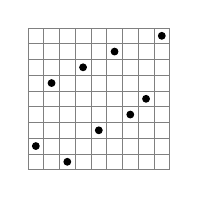
\begin{tikzpicture}[scale=0.2]
% grid
\fill[white]  (0,0) rectangle +(9,9);
\draw[help lines] (0,0) grid +(9,9);
% LTR minima
\filldraw[black] (2.5,0.5) circle (6pt);
\filldraw[black] (4.5,2.5) circle (6pt);
\filldraw[black] (6.5,3.5) circle (6pt);
\filldraw[black] (7.5,4.5) circle (6pt);
\filldraw[black] (8.5,8.5) circle (6pt);
% rest of pts
\filldraw[black] (5.5,7.5) circle (6pt);
\filldraw[black] (3.5,6.5) circle (6pt);
\filldraw[black] (1.5,5.5) circle (6pt);
\filldraw[black] (0.5,1.5) circle (6pt);
\end{tikzpicture}
\caption{\small{An example of a reversible process (left to right) of associating a unique 321-avoider with a given Dyck path.}}
\end{center}
\end{figure}

Having set the scene, we can start the enumeration. Let $\C := \Av(321)$. In a Dyck path, we denote the right step with $\fR$ and the up step with $\fU$. We choose the following combinatorial specification that tracks the right-most point of $\C$ (we do not need to track the left-most point). 
\begin{align*}
  \C^* &= (\C + \EE)\fR\C^*\fU + (\C + \EE)\fR\fU^*\\
  \C &= (\C+\EE)\fR (\C+\EE)\fU.
\end{align*}
In a Dyck path, $\fU$ and $\fR$ are like brackets -- they are interpreted in pairs. Hence, we rewrite the specification into the canonical form~\eqref{eq:combspecav321}. 
\begin{align}
  \begin{aligned}
  \C^* &= \C\C^*\Z + \C^*\Z + \C\Z^* + \Z^*\\
  \C &= \C\C\Z + 2\C\Z + \Z.
\end{aligned}
       \label{eq:combspecav321}
\end{align}
We use this example to demonstrate the method of $\Omega$ operators in full detail. In practice, one would be able to make the analysis that follows significantly shorter by exploiting certain ad-hoc properties of this particular juxtaposition. However, we follow the recipe.

We need to apply $\Omega$ operators to $\Cstar$ in such a way that the expression represents the juxtaposition $\C|\M$, where $\M = \Av(21)$. The \emph{final expression} that represents $\Av(321|21)$ is 
\begin{align}
  \F &= \EE + \M + \frac{\Omega_1(\barCstar) + \Omega_{11}(\barCstar)}{\Z}
      \label{eq:exampleAv321Av21_final}
\end{align}
Indeed, the juxtaposition is either empty (term $\EE$ in $\F$), or the left cell is empty (term $\M$ in $\F$) or both cells are non-empty (terms $\Omega_1(\barCstar)$ and $\Omega_{11}(\barCstar)$ in $\F$ with the former representing a single point in the right cell and the latter representing a sequence of length at least two in the right cell). Notice that the situation where only the right cell is empty cannot occur because the gridline is as far left as possible. Enumeration of $\M$ is trivial and so the main issue will be to enumerate the last two terms of $\F$. The last thing to explain about~\eqref{eq:exampleAv321Av21_final} is the ``division'' by $\Z$ on the RHS. In short, $\Z^{-1}$ removes the phantom point after it is not needed anymore. Indeed, in Lemma~\ref{lem:induction_step} is written with the $\Z$ on the LHS of the identity. This is merely a notational convenience. The enumeration of $\Av(321|21)$ proceeds by obtaining the generating function for $\Omega_1(\barCstar) + \Omega_{11}(\barCstar)$, correcting it by $\Z^{-1}$ to remove phantom points, and then adding to it the generating function for $\EE+\M$. Notice that, in general, any ``algebraic'' post-correction does not affect the character of the generating function (if it was algebraic to begin with). 

Let us first recall the specification of $\barCstar$.
\begin{align*}
  \barCstar &= \Z \ominus \Cstar = \Cstar\Z
\end{align*}
Let $\B$ be the set of all the classes that need to be defined within the combinatorial specification of $\Omega_{11}(\barCstar)$. We start with all the terms in $\F$ inside $\B$, as we need them all to be in the combinatorial specification.
$$\B = \{\EE, \M, \Omega_1(\barCstar), \Omega_{11}(\barCstar)\}$$
We pop $\EE$ first, as it is trivial to define.
\begin{align}
  \EE &= 1
        \label{eq:exampleAv321Av21_E}
\end{align}
Next, we pop $\M$ and define it below.
\begin{align}
  \M &= \Z + \M\Z
       \label{eq:exampleAv321Av21_M}
\end{align}
The new $\B$ is as follows
$$\B = \{\Omega_1(\barCstar), \Omega_{11}(\barCstar)\}.$$
Next we pop $\Omega_1(\barCstar)$ and define it.
\begin{align}
  \begin{aligned}
    \Omega_1(\barCstar) &= \Omega_1(\Cstar\Z)\\
    &= \Omega_1(\Cstar)\Z
  \end{aligned}
  \label{eq:exampleAv321Av21_omega1barCstar}
\end{align}
We update $\B$ to include the new undefined class (in red).
$$\B = \{\textcolor{red}{\Omega_1(\Cstar)}, \Omega_{11}(\barCstar)\}.$$
We pop the new element from $\B$ and define it next. The color coding in~\eqref{eq:exampleAv321Av21_omega1Cstar} and most of the future calculations is there to help the reader trace the origin of the expressions.
\begin{align}
  \begin{aligned}
    \Omega_1(\Cstar) &= \Omega_1(\C\Cstar\Z + \textcolor{orange}{\Cstar\Z} + \textcolor{green}{\C\Z^*} + \textcolor{blue}{\Z^*})\\
    &= \Omega_1(\C)\Omega_0(\Cstar\Z) + \Omega_0(\C)\Omega_1(\Cstar)\Omega_0(\Z) + \textcolor{orange}{\Omega_1(\Cstar)\Omega_0(\Z)} +\\
    &+\textcolor{green}{\Omega_1(\C)\Omega_0(\Z^*) + \Omega_0(\C)\Omega_1(\Z^*)} + \textcolor{blue}{\Omega_1(\Zstar)}\\
    &= \Omega_1(\C)\C\Z + \C\Omega_1(\Cstar)\Z + \textcolor{orange}{\Omega_1(\Cstar)\Z} +\\
    &+\textcolor{green}{\Omega_1(\C)\Z + \C\Z^*\Z} + \textcolor{blue}{\Zstar\Z}
  \end{aligned}
  \label{eq:exampleAv321Av21_omega1Cstar}
\end{align}
We used the facts from Lemma~\ref{lem:ignorance}. For instance, $\Omega_0(\Cstar) = \Omega_0(\C) = \C$. We also used the definitions of $\Omega_1$ and $\Omega_0$, for instance $\Omega_1(\Zstar) = \Zstar\Z$ and $\Omega_0(\Zstar) = \Z$. One term remains undefined on the RHS of~\eqref{eq:exampleAv321Av21_omega1Cstar}, $\Omega_1(\C)$. Since it is the only new class that needs defining, we will skip pushing it to $\B$ and then immediately popping it out of there. The definition is below.
\begin{align}
  \begin{aligned}
    \Omega_1(\C) &= \Omega_1(\C\C\Z + \textcolor{orange}{2\C\Z} + \textcolor{green}{\Z})\\
    &= \Omega_1(\C)\C\Z + \C\Omega_1(\C)\Z + \C\C\Z^*\Z + \textcolor{orange}{2\Omega_1(\C)\Z + 2\C\Z^*\Z} + \textcolor{green}{\Z^*\Z}
  \end{aligned}
  \label{eq:exampleAv321Av21_omega1C}
\end{align}
There is no undefined term on the RHS of~\eqref{eq:exampleAv321Av21_omega1C} and therefore $\B$ is currently a singleton.
$$\B = \{\Omega_{11}(\barCstar)\}$$
Therefore, we define the only class in $\B$.
\begin{align}
  \begin{aligned}
  \Omega_{11}(\barCstar) &= \Omega_{11}(\Cstar\Z)\\
                         &= \Omega_{11}(\Cstar)\Z + \Omega_{10}(\Cstar)\Omega_{01}(\Z)\\
                         &= \Omega_{11}(\Cstar)\Z + \Omega_{10}(\Cstar)(\M+\EE)\Z^*\Z\\
                       \end{aligned}
  \label{eq:omega11barCstar}
\end{align}
We update $\B$ according to the last line above (recall that $\M$ is already defined in~\eqref{eq:exampleAv321Av21_M}). Both items are new.
$$\B = \{\textcolor{red}{\Omega_{11}(\Cstar), \Omega_{10}(\Cstar)}\}.$$

Before we proceed, we remark that if an expression is not an argument to any $\Omega_i$, i.e. it is a \emph{top-level expression}, then it can be evaluated. In what follows, we will immediately evaluate all top-level expressions as far as is convenient. Notice that, because we only apply one layer of $\Omega$ operators to any original class ($\C,\Cstar,\M,\Z,\Zstar$), all our expressions are top-level.

We pop $\Omega_{11}(\Cstar)$ out of $\B$ to define it below.
\begin{align}
  \begin{aligned}
  \Omega_{11}(\Cstar) &= \Omega_{11}(\C\Cstar\Z+ \textcolor{orange}{\Cstar\Z} + \textcolor{green}{\C\Z^*} + \textcolor{blue}{\Z^*})\\
                      &= \Omega_{11}(\C\Cstar\Z) + \textcolor{orange}{\Omega_{11}(\Cstar\Z)} + \textcolor{green}{\Omega_{11}(\C\Z^*)} + \textcolor{blue}{\Omega_{11}(\Z^*)}\\
                      &= \Omega_{11}(\C)\Omega_0(\Cstar)\Omega_0(\Z) + \Omega_0(\C)\Omega_{11}(\Cstar)\Omega_0(\Z) +\\
                      &+ \Omega_{10}(\C)\Omega_{01}(\Cstar)\Omega_0(\Z) + \Omega_{10}(\C)\Omega_\infty(\Cstar)\Omega_{01}(\Z) +\\
                      &+ \Omega_0(\C)\Omega_{10}(\Cstar)\Omega_{01}(\Z) + \textcolor{orange}{\Omega_{11}(\Cstar)\Omega_0(\Z) + \Omega_{10}(\Cstar)\Omega_{01}(\Z)} +\\
                      &+ \textcolor{green}{\Omega_{11}(C)\Omega_0(\Z^*) + \Omega_0(\C)\Omega_{11}(\Z^*) + \Omega_{10}(\C)\Omega_{01}(\Z^*)} +\\
                      &+ \textcolor{blue}{\Omega_{11}(\Z^*)}\\
                      &= \Omega_{11}(\C)\C\Z + \C\Omega_{11}(\Cstar)\Z + \Omega_{10}(\C)\Omega_{01}(\Cstar)\Z +\\
                      &+ \Omega_{10}(\C)\Omega_\infty(\C)(\M+\EE)\Z^*\Z +\C\Omega_{10}(\Cstar)(\M+\EE)\Z^*\Z + \\
                      &+ \textcolor{orange}{\Omega_{11}(\Cstar)\Z + \Omega_{10}(\Cstar)(\M+\EE)\Z^*\Z} +\\
                      &+ \textcolor{green}{\Omega_{11}(\C)\Z + \C\Z(\M+\EE)\Z^*\Z + \Omega_{10}(\C)(\M+\EE)\Z^*\Z} +\\
                      &+\textcolor{blue}{\Z(\M+\EE)\Z^*\Z}\\
                      %&= \textcolor{blue}{\M\Z^*\Z} + \textcolor{green}{\Omega_{11}(\C)\Z} + \textcolor{green}{\Omega_{10}(\C)\M^*\Z} + \textcolor{green}{\C\M\Z^*\Z} + \textcolor{orange}{\Omega_{11}(\Cstar)\Z} + \textcolor{orange}{\Omega_{10}(\Cstar)\M^*\Z} +\\
                      %&+ \Omega_{11}(\C)\C\Z + \Omega_{10}(\C)\Omega_\infty(\C)\M^*\Z + \C\Omega_{10}(\Cstar)\M^*\Z + \C\Omega_{11}(\Cstar)\Z + \Omega_{10}(\C) \Omega_{01}(\C)\Z
                    \end{aligned}
                        \label{eq:exampleAv321Av21_omega11Cstar}
\end{align}
Updating $\B$ yields the following list. The red items those that have not yet been defined and occur on the RHS of~\eqref{eq:exampleAv321Av21_omega11Cstar}.
$$\B = \{\Omega_{10}(\Cstar),\textcolor{red}{\Omega_\infty(\C)}, \textcolor{red}{\Omega_{11}(\C)},\textcolor{red}{\Omega_{10}(\C)}, \textcolor{red}{\Omega_{01}(\C)}, \textcolor{red}{\Omega_{01}(\Cstar)}\}$$
Before we proceed, we define $\Omega_\infty(\C)$ as, in the scheme of things, it is a trivial task.
\begin{align}
  \begin{aligned}
    \Omega_\infty(\C) &= \Omega_\infty(\C)\Omega_\infty(\C)\Omega_\infty(\Z) + 2\Omega_\infty(\C)\Omega_\infty(\Z) + \Omega_\infty(\Z))\\
    &= \Omega_\infty(\C)^2(\M+\EE)\Z + 2\Omega_\infty(\C)(\M+\EE)\Z + (\M+\EE)\Z
  \end{aligned}
  \label{eq:exampleAv321Av21_omegainftyC}
\end{align}
Notice that $\Omega_\infty(\C)$ is essentially class $\C$ where every atom/point is replaced with a nonempty sequence of points. Indeed, the generating function of $\Omega_\infty(\C)$ is $C(z/(1-z)$, where $C(z)$ is the generating function of $\C$. Having defined $\Omega_\infty(\C)$, we can reduce what are essentially duplicities in $\B$ by applying Lemma~\ref{lem:ignorance}. This allows us to disregard $\Omega_{01}(\Cstar)$ and only keep $\Omega_{01}(\C)$. The new $\B$ is below.
$$\B = \{\Omega_{10}(\Cstar), \textcolor{red}{\Omega_{11}(\C)},\textcolor{red}{\Omega_{10}(\C)}, \textcolor{red}{\Omega_{01}(\C)}\}$$
Next, pop $\Omega_{10}(\Cstar)$ out of $\B$. To speed up the procedure, we apply Lemma~\ref{lem:ignorance} to the expressions below as soon as we can. This way there will not be any need to post-adjust $\B$. 
\begin{align}
  \begin{aligned}
  \Omega_{10}(\Cstar) &= \Omega_{10}(\C\Cstar\Z + \textcolor{orange}{\Cstar\Z} + \textcolor{green}{\C\Z^*} + \textcolor{blue}{\Z^*})\\
                      &= \Omega_{10}(\C)\Omega_\infty(\C)(\M+\EE)\Z + \C\Omega_{10}(\Cstar)(\M+\EE)\Z\\ % + \C\C\Z(\M+\EE)\Z +\\
                      &+\textcolor{orange}{\Omega_{10}(\Cstar)(\M+\EE)\Z}+\\ %+ \C\Z(\M+\EE)\Z} +\\
                      &+\textcolor{green}{\Omega_{10}(\C)(\M+\EE)\Z + \C\Z(\M+\EE)\Z} +\\
                      &+\textcolor{blue}{\Z(\M+\EE)\Z}
                    \end{aligned}
                        \label{eq:exampleAv321Av21_omega10Cstar}
\end{align}
We do not augment $\B$ at all after this definition as everything on the RHS has either been defined or is already in $\B$. Therefore, we have
$$\B = \{\Omega_{11}(\C),\Omega_{10}(\C), \Omega_{01}(\C)\}.$$
We pop $\Omega_{11}(\C)$ and define it below.
\begin{align}
  \begin{aligned}
    \Omega_{11}(\C) &= \Omega_{11}(\C\C\Z + \textcolor{orange}{2\C\Z} + \textcolor{green}{\Z})\\
    &= \Omega_{11}(\C)\C\Z + \C\Omega_{11}(\C)\Z + \C\C\Z(\M+\EE)\Z^*\Z + \Omega_{10}(\C)\Omega_{01}(\C)\Z +\\
    &+ \Omega_{10}(\C)\Omega_\infty(\C)(\M+\EE)\Z^*\Z + \C\Omega_{10}(\C)(\M+\EE)\Z^*\Z +\\
    &+ \textcolor{orange}{2\Omega_{11}(\C)\Z + 2\C\Z(\M+\EE)\Z^*\Z + 2\Omega_{10}(\C)(\M+\EE)\Z^*\Z} +\\
    &+\textcolor{green}{\Z(\M+\EE)\Z^*\Z}\\
  \end{aligned}
  \label{eq:exampleAv321Av21_omega11C}
\end{align}
Again, there is nothing in the definition~\eqref{eq:exampleAv321Av21_omega11C} which would not be known or already in $\B$. We do not augment $\B$ and it remains as it was.
$$\B = \{\Omega_{10}(\C), \Omega_{01}(\C)\}$$
We pop the next item, $\Omega_{10}(\C)$.
\begin{align}
  \begin{aligned}
    \Omega_{10}(\C) &= \Omega_{10}(\C\C\Z + \textcolor{orange}{2\C\Z} + \textcolor{green}{\Z})\\
    &= \Omega_{10}(\C)\Omega_\infty(\C)(\M+\EE)\Z + \C\Omega_{10}(\C)(\M+\EE)\Z +\\
    &+ \C\C\Z(\M+\EE)\Z +\\
    &+ \textcolor{orange}{2\Omega_{10}(\C)(\M+\EE)\Z + 2\C\Z(\M+\EE)\Z} + \textcolor{green}{\Z(\M+\EE)\Z}
  \end{aligned}
  \label{eq:exampleAv321Av21_omega10C}
\end{align}
In~\eqref{eq:exampleAv321Av21_omega10C} we do not require any new items. In fact, it turns out that $\Omega_{10}(\C)$ is computable from its own definition only, a standalone recursion. There is only one class left in $\B$.
$$\B = \{\Omega_{01}(\C)\}$$
We pop the last item from $\B$, $\Omega_{01}(\C)$.
\begin{align}
  \begin{aligned}
    \Omega_{01}(\C) &= \Omega_{01}(\C\C\Z + \textcolor{orange}{2\C\Z} + \textcolor{green}{\Z})\\
    &= \Omega_{01}(\C)\C\Z + \Omega_\infty(\C)\Omega_{01}(\C)\Z + \Omega_\infty(\C)\Omega_\infty(\C)(\M+\EE)\Z^*\Z +\\
    &+ \textcolor{orange}{2\Omega_{01}(\C)\Z + 2\Omega_\infty(\C)(\M+\EE)\Z^*\Z} + \textcolor{green}{(\M+\EE)\Z^*\Z}
  \end{aligned}
  \label{eq:exampleAv321Av21_omega01C}
\end{align}
As there is nothing in $\B$ and we do not augment it after~\eqref{eq:exampleAv321Av21_omega01C}, the definition of $\Omega_{11}(\barCstar)$ is self-contained assuming that we include definitions~\eqref{eq:exampleAv321Av21_E}, \eqref{eq:exampleAv321Av21_M}, \eqref{eq:exampleAv321Av21_omega1barCstar}, \eqref{eq:exampleAv321Av21_omega1Cstar}, \eqref{eq:exampleAv321Av21_omega1C}, \eqref{eq:omega11barCstar}, \eqref{eq:exampleAv321Av21_omega11Cstar}, \eqref{eq:exampleAv321Av21_omegainftyC}, \eqref{eq:exampleAv321Av21_omega10Cstar}, \eqref{eq:exampleAv321Av21_omega11C}, \eqref{eq:exampleAv321Av21_omega10C}, and \eqref{eq:exampleAv321Av21_omega01C}.

The corresponding calculations are done in Mathematica~\cite{mathematica} and can be found in \texttt{exampleAv321Av21.nb} inside the \texttt{scripts} folder at

$$\href{https://github.com/jsliacan/thesis}{\texttt{https://github.com/jsliacan/thesis}}.$$

The gerating function of $\Av(321|21)$ coincides with the one obtained in Section~\ref{sec:catalanjuxt_av321av21} and we restate it below for convenience.
\begin{align*}
  F(z) &= -\frac{1-\sqrt{1-4z} + z(-4+\sqrt{1-4z} + \sqrt{1-5z}/\sqrt{1-z})}{2z^2}
\end{align*}
The first twelve term sof the counting sequence enumerating $\Av(321|21)$ are
$$1,1,2,6,23,98,434,1949,8803,39888,181201,825201,3767757.$$
The sequence is in the OEIS~\cite{oeis} as \href{https://oeis.org/A278301}{A278301}.
\subsection{Example: $\Av(21|21|21)$}
\label{sec:example_mmm}
As before, $\Av(21)$ denotes the class of increasing permutations and $\Av(21|21|21)$ then refers to a juxtaposition of $\Av(21)$ with $\Av(21)$, and then the resulting class juxtaposed with $\Av(21)$ (on the right). We know that $\Av(21)$, and its non-empty version that we call $\M$, are context-free classes and clearly admit combinatorial specifications that track the right-most point. This example is a very simple yet not completely degenerate case of iterated juxtapositions with at least three cells. We choose to give full details of enumeration to illustrate how our methods work on repeated juxtapositions. While it is entirely possible to enumerate this class by following the algorithmic definitions in Section~\ref{sec:iterjuxt_main}, we exploit the slight degeneracies in this example to shorten the write-up.

First of all, we rewrite $\Av(21|21|21)$ in terms of $\Omega$ operators (defined in Section~\ref{sec:iterjuxt_intro}). Because we choose the gridding with gridlines as far left as possible (gridding from the right), every griddable permutation is griddable in one of the following ways: either all three cells are non-empty, or only the leftmost cell is empty, or only the rightmost cell is non-empty, or all three cells are empty. If all three cells are empty, this case is represented by the empty class $\EE$. If the leftmost two cells are empty, this is essentially the monotone increasing class $\M$ (non-empty, as before). For the remaining cases, observe that the rightmost juxtaposition does not need to track the rightmost point as nothing further will be juxtaposed on its right. Therefore, at the outermost layer, we are only interested in expressions of the form $\Omega_{10}(\M)$ and $\Omega_{10}(\M|\M)$  (when one and zero cells are empty, respectively). Consider the case when the leftmost cell is empty and the remaining two cells are non-empty. We express this situation by $\Omega_{10}(\Mstar)(\M+\EE)$ --- the left of the two cells is a non-empty monotone increasing class whose combinatorial specification tracks the rightmost point, $\Mstar$ (defined in~\eqref{eq:mmm_Mstar}). The term $(\M+\EE)$ makes sure that we allow the right cell to place points above everything in the left cell. We either use a phantom point or need the term $(\M+\EE)$ to place points above the topmost point on the LHS. The other case is when all three cells are nonempty. Then we need to use the phantom point and track the rightmost point in the middle cell. So, the middle cell can have a single point or a sequence of length at least two. Therefore, the first two cells are either $\Omega_1(\barMstar)$ or $\Omega_{11}(\barMstar)$. We then apply $\Omega_{10}$ to them. Notice that we do not multiply by $\M+\EE$ as we are already using the phantom point. Consequently, we remove the trace of the phantom point by dividing the 3-cell expression by $\Z$. Therefore, the final object that we aim to enumerate is $\F$ below.


\begin{align}
  \F &= \EE + \M + (\M+\EE)\Omega_{10}(\Mstar) +\frac{1}{\Z}(\Omega_{10}(\Omega_1(\barMstar)) + \Omega_{10}(\Omega_{11}(\barMstar)))
\label{eq:mmm_final}
\end{align}
Notice that $\F$ is not a class or a combinatorial specification of a class. It is merely an expression that is formally correct and captures both structure and enumeration of $\Av(21|21|21)$. It is a sort of hybrid benefiting from both the combinatorial specification and the generating function of $\Av(21|21|21)$. Therefore, we will handle~\eqref{eq:mmm_final} term by term. The ``division'' in the last term will be resolved in a manner similar to that in Lemma~\ref{lem:induction_step} or Section~\ref{sec:example_Av321Av21} --- we will enumerate $\Omega_{10}(\Omega_1(\barMstar)) + \Omega_{10}(\Omega_{11}(\barMstar))$ and remove the phantom point afterwards. 
% \begin{align}
%   \EE + \M + (\M+\EE)\Omega_{10}(\Mstar) +\Omega_{10}(\Omega_1(\barMstar)) + \Omega_{10}(\Omega_{11}(\barMstar)).
%   \label{eq:mmm_combspec}
% \end{align}
% Once we have it, we obtain its generating function and at this stage, we remove the trace of the phantom point by dividing the appropriate terms by $\Z$.

We begin by defining the most simple classes so that we do not have to worry about them later. 
\begin{align}
  \M &= \Z + \M\Z \label{eq:mmm_m}\\
  \Mstar &=  \Zstar + \M\Zstar \label{eq:mmm_Mstar}\\
  \barMstar &= \Mstar\Z \label{eq:mmm_barMstar}\\
  \Omega_0(\M)&= \Z + \M\Z = \M\label{eq:mmm_omega0M}\\
  \Omega_0(\Mstar) &= \Z + \M\Z = \M\label{eq:mmm_omega0Mstar}
\end{align}
We will often use the fact that $(\M+\EE)\Z = \M$, such as in~\eqref{eq:mmm_omega0M} and~\eqref{eq:mmm_omega0Mstar}. We also use it to collapse $\Omega_\infty(\Zstar)$ into $\M$ as follows: $\Omega_\infty(\Zstar) = (\M+\EE)\Z = \M$. First, define $\Omega_\infty(\M)$. 
\begin{align}
  \begin{aligned}
    \Omega_\infty(\M) &= \Omega_\infty(\Z) + \Omega_\infty(\M)\Omega_\infty(\Z)\\
    &= \M + \Omega_\infty(\M)\M
  \end{aligned}
      \label{eq:mmm_omegainfty}
\end{align}

Next, we define the terms with two nonempty cells.

\begin{align}
  \begin{aligned}
    \Omega_{10}(\M) &= \Omega_{10}(\Z) + \Omega_{10}(\M\Z)\\
    &= \Omega_{10}(\Z) + \Omega_{10}(M)\Omega_\infty(\Z) + \Omega_0(\M)\Omega_{10}(\Z)\\
    &= \M\Z + \Omega_{10}(\M)\M + \M\M\Z
  \end{aligned}
      \label{eq:mmm_omega10M}
\end{align}

\begin{observation}
\label{mmm_observation}
Notice that $\Omega_{10}$ has the same effect on $\M$ as on $\Mstar$, i.e. $\Omega_{10}(\Mstar) = \Omega_{10}(\M)$. This is quite peculiar as $\Omega_{10}$ does not ignore the rightmost point in its argument. However, in $\M$ and $\Mstar$, the rightmost point is also the topmost point. And hence every point in $\M$ and $\Mstar$ is below the rightmost point. By the same reasoning, $\Omega_1(\Mstar) = \Omega_1(\M)$ and $\Omega_{11}(\Mstar) = \Omega_{11}(\M)$. We will use these identities below to avoid defining expressions duplicitously.
\end{observation}
We have now defined every class needed for the first three terms of~\eqref{eq:mmm_final}. Next, we define the terms that represent the three nonempty cells with a phantom point above the first cell. As in Section~\ref{sec:example_Av321Av21}, let $\B$ be the stack of undefined items. We begin with
$$\B = \{\Omega_{10}(\Omega_1(\barMstar)) + \Omega_{10}(\Omega_{11}(\barMstar))\}.$$
Since we have defined $\barMstar$ in~\eqref{eq:mmm_barMstar}, we now need to push $\Omega_1(\barMstar)$ and $\Omega_{11}(\barMstar)$ onto the stack before we define anything else. Hence,
$$\B = \{\textcolor{red}{\Omega_1(\barMstar), \Omega_{11}(\barMstar)}, \Omega_{10}(\Omega_1(\barMstar)), \Omega_{10}(\Omega_{11}(\barMstar))\}.$$
We pop the first item and define it below.
\begin{align}
  \begin{aligned}
  \Omega_1(\barMstar) &= \Omega_1(\Mstar)\Omega_0(\Z)\\
                      &=  \Omega_1(\M)\Z
                    \end{aligned}
\end{align}
Recall that $\Omega_1(\Mstar)$ is the same object as $\Omega_1(\M)$ thanks to the Observation~\ref{mmm_observation}, that the rightmost point is also the topmost point in $\M$. Therefore, we need to define $\Omega_1(\M)$. We skip pushing and popping it onto and from the stack and define it straight away.
% \begin{align}
% \Omega_1(\Mstar) &= \Omega_1(\M)
% \label{eq:omega1Mstar}
% \end{align}
\begin{align}
  \begin{aligned}
    \Omega_1(\M) &= \Omega_1(\Z + \M\Z)\\
    &= \Omega_1(\Z) + \Omega_1(\M)\Omega_0(\Z) + \Omega_0(\M)\Omega_1(\Z)\\
    &= \Zstar\Z + \Omega_1(\M)\Z + \M\Zstar\Z
  \end{aligned}
\end{align}
Currently, $\B$ looks as follows
$$\B = \{\Omega_{11}(\barMstar), \Omega_{10}(\Omega_1(\barMstar)), \Omega_{10}(\Omega_{11}(\barMstar))\}.$$
We pop the next element and break it down.
\begin{align}
  \begin{aligned}
    \Omega_{11}(\barMstar) &= \Omega_{11}(\Mstar\Z)\\
    &= \Omega_{11}(\Mstar)\Omega_0(\Z) + \Omega_{10}(\Mstar)\Omega_{01}(\Z)\\
    &= \Omega_{11}(\Mstar)\Z + \Omega_{10}(\Mstar)\M\Z
  \end{aligned}
\end{align}
Where the last line follows from the definition of $\Omega_{0}$ and $\Omega_{01}$ and from the fact that $(\M+\EE)\Z = \M$. Given that $\Omega_{11}(\Mstar) = \Omega_{11}(\M)$ and $\Omega_{10}(\Mstar) = \Omega_{10}(\M)$, we push the only new element $\Omega_{11}(\M)$ onto $\B$ (recall that $\Omega_{10}(\M)$ was defined in~\eqref{eq:mmm_omega10M}).
$$\B = \{\textcolor{red}{\Omega_{11}(\M)}, \Omega_{10}(\Omega_1(\barMstar)), \Omega_{10}(\Omega_{11}(\barMstar))\}$$
We pop $\Omega_{11}(\M)$ next.
\begin{align}
  \begin{aligned}
    \Omega_{11}(\M) &= \Omega_{11}(\Z) + \Omega_{11}(\M)\Omega_0(\Z) + \Omega_0(\M)\Omega_{11}(\Z) +\\
    &+\Omega_{10}(\M)\Omega_{01}(\Z)\\
    &= \M\Zstar\Z + \Omega_{11}(\M)\Z + \M\M\Zstar\Z + \Omega_{10}(\M)\Mstar\Z
  \end{aligned}
      \label{eq:mmm_omega11M}
\end{align}
We used the definition of $\Omega_{11}$, $\Omega_{0}$ and $\Omega_{01}$ to evaluate them on the base case input $\Z$. There is no new class on the last line of~\eqref{eq:mmm_omega11M} and hence we need not update $\B$ which now is
$$\B = \{\Omega_{10}(\Omega_1(\barMstar)), \Omega_{10}(\Omega_{11}(\barMstar))\}.$$
Notice that we now know both inner expressions of the items in $\B$: $\Omega_1(\barMstar)$ and $\Omega_{11}(\barMstar)$. It therefore remains to define the action of $\Omega_{10}$ on them. We pop the next item from $\B$.
\begin{align}
  \begin{aligned}
  \Omega_{10}(\Omega_1(\barMstar)) &= \Omega_{10}(\Omega_1(\Mstar)\Omega_0(\Z))\quad \text{by~\eqref{eq:mmm_barMstar}}\\
                                   &= \Omega_{10}(\Omega_1(\Mstar))\Omega_\infty(\Omega_0(\Z))\quad \text{by def of $\Omega_{10}$}\\
                                   &= \Omega_{10}(\Omega_1(\M))\M
                                   \end{aligned}
\end{align}
where the last line follows from $\Omega_\infty(\Omega_0(Z)) = \Omega_\infty(\Z) = \M$ and $\Omega_{10}(\Omega_1(\Mstar)) = \Omega_{10}(\Omega_1(\M))$ by Observation~\ref{mmm_observation}. Given that again we only have one new term to be defined, we omit pushing and popping it to and from $\B$. Therefore,
\begin{align}
  \begin{aligned}
    \Omega_{10}(\Omega_1(\M)) &= \Omega_{10}(\Omega_1(\Z)) + \textcolor{orange}{\Omega_{10}(\Omega_1(\M)\Omega_0(\Z))} + \textcolor{green}{\Omega_{10}(\Omega_0(\M)\Omega_1(\Z))}\\
    &= \Omega_{10}(\Zstar)\Omega_\infty(\Z) + \textcolor{orange}{\Omega_{10}(\Omega_1(\M))\Omega_\infty(\Omega_0(\Z))} +\\
    &+ \textcolor{green}{\Omega_{10}(\Omega_0(\M))\Omega_\infty(\Zstar\Z) + \Omega_0(\Omega_0(\M))\Omega_{10}(\Zstar)\Omega_\infty(\Z)}\\
    &= \M\Z\M + \textcolor{orange}{\Omega_{10}(\Omega_1(\M))\M} + \textcolor{green}{\Omega_{10}(\M)\M\M + \M\M\Z\M}
  \end{aligned}
      \label{eq:mmm_omega101M}
\end{align}
There are no undefined objects in the last line and hence $\B$ is now a singleton: it remains to define $\Omega_{10}(\Omega_{11}(\barMstar))$. 
\begin{align}
  \begin{aligned}
\Omega_{10}(\Omega_{11}(\barMstar)) &= \Omega_{10}(\Omega_{11}(\Mstar\Z))\quad\\
                                    &= \Omega_{10}(\Omega_{11}(\Mstar)\Omega_0(\Z)) + \Omega_{10}(\Omega_{10}(\Mstar)\Omega_{01}(\Z)) \\
                                    &= \Omega_{10}(\Omega_{11}(\Mstar))\Omega_\infty(\Omega_0(\Z)) +\\
                                    &+ \textcolor{orange}{\Omega_{10}(\Omega_{10}(\Mstar))\Omega_\infty(\Omega_{01}(\Z))} + \textcolor{green}{\Omega_0(\Omega_{10}(\Mstar))\Omega_{10}(\Omega_{01}(\Z))}\\
                                    &= \Omega_{10}(\Omega_{11}(\M))\M + \textcolor{orange}{\Omega_{10}(\Omega_{10}(\M))\Omega_\infty(\M)\M} +\\
                                    &+ \textcolor{green}{\Omega_{10}(\M)\Omega_{10}(\M)\M} \\
  \end{aligned}
\label{eq:mmm_lastterm}
\end{align}
The first three equalities above follow from the definitions of $\barMstar$, $\Omega_{11}$, and $\Omega_{10}$, respectively. The last equality evaluates as many expressions as possible. We used facts from Observation~\ref{mmm_observation}: $\Omega_{11}(\Mstar) = \Omega_{11}(\M)$ and $\Omega_{10}(\Mstar)=\Omega_{10}(\M)$, as well as the definitions of $\Omega_0, \Omega_\infty, \Omega_{01}, \Omega_{10}$ on the base case input $\Z$. However, for~\eqref{eq:mmm_lastterm} to be well-defined, we need to include the following set of expressions in the combinatorial specification: $$\B = \{\Omega_{10}(\Omega_{10}(\M)), \Omega_{10}(\Omega_{11}(\M))\}.$$
We pop the top item and define it below.
\begin{align}
  \begin{aligned}
    \Omega_{10}(\Omega_{10}(\M)) &= \Omega_{10}(\M\Z + \textcolor{orange}{\Omega_{10}(\M)\M} + \textcolor{green}{\M\M\Z})\\
    &= \Omega_{10}(\M)\Omega_\infty(\Z) + \Omega_0(\M)\Omega_{10}(\Z) +\\
    &+ \textcolor{orange}{\Omega_{10}(\Omega_{10}(\M))\Omega_\infty) + \Omega_0(\Omega_{10}(\M))\Omega_{10}(\M)} +\\
    &+ \textcolor{green}{\Omega_{10}(\M)\Omega_\infty(\M\Z) + \Omega_0(\M)\Omega_{10}(\M)\Omega_\infty(\Z)} +\\
    &+ \textcolor{green}{\Omega_0(\M\M)\Omega_{10}(\Z)}\\
    &= \Omega_{10}(\M)\M + \M\M\Z + \textcolor{orange}{\Omega_{10}(\Omega_{10}(\M))\Omega_\infty(\M)} +\\
    &+ \textcolor{orange}{\Omega_{10}(\M)\Omega_{10}(\M)} + \textcolor{green}{\Omega_{10}(\M)\Omega_\infty(\M)\M} +\\
    &+ \textcolor{green}{\M\Omega_{10}(\M)\M + \M\M\M\Z}
  \end{aligned}
      \label{eq:mmm_omega1010M}
\end{align}
Since everything in~\eqref{eq:mmm_omega1010M} is either already known or in $\B$, which currently contains only one element
$$\B = \{\Omega_{10}(\Omega_{11}(\M))\}.$$
Let us now define $\Omega_{10}(\Omega_{11}(\M))$. 
\begin{align}
  \begin{aligned}
    \Omega_{10}(\Omega_{11}(\M)) &= \Omega_{10}(\M\Zstar\Z) + \textcolor{orange}{\Omega_{10}(\Omega_{11}(\M)\Z)} + \textcolor{green}{\Omega_{10}(\M\M\Zstar\Z)} +\\
    &+\textcolor{blue}{\Omega_{10}(\Omega_{10}(\M)\Mstar\Z)}\\
    &= \Omega_{10}(\M)\Omega_\infty(\Zstar\Z) + \M\Omega_{10}(\Zstar)\Omega_\infty(\Z) +\\
    &+ \textcolor{orange}{\Omega_{10}(\Omega_{11}(\M))\Omega_\infty(\Z)} +\\
    &+ \textcolor{green}{\Omega_{10}(\M)\Omega_\infty(\M\Zstar\Z) + \M\Omega_{10}(\M)\Omega_\infty(\Zstar\Z) +}\\
    &+ \textcolor{green}{\M\M\Omega_{10}(\Zstar)\Omega_\infty(\Z)}\\
    &+ \textcolor{blue}{\Omega_{10}(\Omega_{10}(\M))\Omega_\infty(\Mstar\Z) + \Omega_0(\Omega_{10}(\M))\Omega_{10}(\Mstar)\Omega_\infty(\Z)}\\
    &= \Omega_{10}(\M)\M\M + \M\M\Z\M + \textcolor{orange}{\Omega_{10}(\Omega_{11}(\M))\M} +\\
    &+ \textcolor{green}{\Omega_{10}(\M)\Omega_\infty(\M)\M\M + \M\Omega_{10}(\M)\M\M} +\\
    &+ \textcolor{green}{\M\M\M\Z\M} +\\
    &+ \textcolor{blue}{\Omega_{10}(\Omega_{10}(\M))\Omega_\infty(\M)\M + \Omega_{10}(\M)\Omega_{10}(\M)\M}
  \end{aligned}
      \label{eq:mmm_omega1011M}
\end{align}
Now, everything in the last line of~\eqref{eq:mmm_omega1011M} has already been defined. Hence, with the information in~\eqref{eq:mmm_m}--\eqref{eq:mmm_omega1011M}, we transform~\eqref{eq:mmm_final} into the following expression.
\begin{align}
  \begin{aligned}
  &\EE + \M + (\M + \EE)\Omega_{10}(\M) +1/\Z\bigg(\Omega_{10}(\Omega_1(\M))\M +\\
     &+\Omega_{10}(\Omega_{11}(\M))\M +\Omega_{10}(\Omega_{10}(\M))\Omega_\infty(\M)\M + \Omega_{10}(\M)\Omega_{10}(\M)\M\bigg)
   \end{aligned}
\label{eq:mmm_combspec_final}
\end{align}
From~\eqref{eq:mmm_combspec_final} we see that not all our definitions need to be included in the ``combinatorial specification''~\eqref{eq:mmm_final}. It turns out that some can be skipped as we managed to express their content directly through lower-level operators. In particular, we need to include the following definitions in our combinatorial specification: $\M$~\eqref{eq:mmm_m}, $\Omega_\infty(\M)$~\eqref{eq:mmm_omegainfty}, $\Omega_{10}(\M)$~\eqref{eq:mmm_omega10M}, $\Omega_{10}(\Omega_1(\M))$~\eqref{eq:mmm_omega101M}, $\Omega_{10}(\Omega_{10}(\M))$~\eqref{eq:mmm_omega1010M}, and $\Omega_{10}(\Omega_{11}(\M))$~\eqref{eq:mmm_omega1011M}. However, recall despite ``division'' being an illegal operation, it is simply our notation for removing the added phantom point from every single permutation in $\Av(21|21|21)$. This is expressed in~\eqref{eq:mmm_combspec_final} whose formal meaning is valid and represents the class $\Av(21|21|21)$. Therefore, the generating function of $\F$ stores the counting sequence enumerating $\Av(21|21|21)$.

The relevant Mathematica script implementing enumeration of $\Av(21|21|21)$ via the process described in this section can be found in \texttt{exampleMMM.nb}. The file resides in the \texttt{scripts} folder of the accompanying thesis repository at

\begin{center}\href{https://github.com/jsliacan/thesis}{\texttt{https://github.com/jsliacan/thesis}}.\end{center}

The generating function of $\Av(21|21|21)$ is
\begin{align}
  F(z) &= \frac{22x^5-52x^4+56x^3-32x^2+9x-1}{(x-1)^3(2x-1)^2(3x-1)}.
\end{align}
The counting sequence that we obtain for the number of permutations in $\Av(21|21|21)$ of length $k=0,\ldots,12$ is $$1, 1, 2, 6, 23, 93, 360, 1312, 4541, 15111, 48854, 154674, 482355\ldots$$
This agrees with Bevan's enumeration of $\Av(21|21|21)$ in his thesis~\cite{bevan2015thesis}, Part I, Table 3.1. The sequence is not in the OEIS~\cite{oeis}.

\subsection{Example: Separable next to monotone}
\label{sec:example_sepav21}
The class of separable permutations has finitely many simple permutations and is relatively simple. We still think this example is useful in that it demonstrates that our method can be used to enumerate various juxtapositions exactly. To the best of our knowledge, the juxtaposition class $\S|\M$, where $\M$ is an increasing monotone class, has not been enumerated yet. We juxtapose $\M$ on the right of the class of separable permutations $\S$ and choose to work with the following combinatorial specification of $\S$.
\begin{align}
  \begin{aligned}
    \S^* &= \Z^* + \S_{\oplus}\S^* + \S^*\S_{\ominus}\\
    \S &= \Z + \S_{\oplus}\S + \S\S_{\ominus}\\
    \S_{\ominus} &= \Z + \S_\oplus\S\\
    \S_\oplus &= \Z + \S\S_\ominus.
    \label{eq:sepav21_sep}
  \end{aligned}
\end{align}
We also know that
\begin{align}
  \begin{aligned}
    \M &= \Z + \M\Z\\
    \Mstar &= \Zstar + \M\Zstar
  \end{aligned}
\end{align}
Before we proceed with the enumeration, notice that whether $\M$ is a monotone increasing or a monotone decreasing class, $\S|\M$ is enumerated by the same generating function. This is obvious from the chosen combinatorial specification~\eqref{eq:sepav21_sep}. Indeed, if $\M$ is monotone decreasing, we flip the entire juxtaposition around a horizontal axis (so that it is upside down). The main observation is that if $\pi \in \S$, then a ``flip'' of $\pi$ around the horizontal axis is also in $\S$. This is easy to verify. Therefore, in case of decreasing $\M$, we enumerate the upside down juxtaposition.

Back to the example with a monotone increasing $\M$. To make this example as short as possible, we will not write out the whole derivation of expressions in the combinatorial specification. It is a routine process which could, in principle, be automated. Also, instead of keeping track of a set $\B$ of classes that we need to define, we will determine the whole list of classes that we need ahead of time. Then we just define the classes in that list.

Notice that we will not need to define $\Sstar_\oplus$ or $\Sstar_\ominus$. This is because $\S_\oplus$ and $\S_\ominus$, the way they are used in~\eqref{eq:sepav21_sep}, can never contain the rightmost point. Refer to the pictorial definition~\eqref{eq:sepstar} of $\S$ for a clearer image. Moreover, notice that
\begin{align*}
  \Omega_0(\Sstar) &= \Omega_0(\S)\\
  \Omega_\infty(\Sstar) &= \Omega_\infty(\S)\\
  \Omega_{01}(\Sstar) &= \Omega_{01}(\S).
\end{align*}
All of these operators ignore and erase the rightmost points of their arguments. Hence, it does not matter if we feed them $\Sstar$ or $\S$. Moreover, $\Omega_0(\S) = \S$, and therefore $\Omega_0(\Sstar) = \S$ as well. We are left with Table~\ref{tab:sep_todefine} of items (combinations of arguments and operators) that we need to define in the combinatorial specification of $\S$.
\begin{table}[ht]
  \centering
  \begin{tabular}{l|c c c c}
    & $\S$ & $\Sstar$ & $\S_\ominus$ & $\S_\oplus$\\
    \hline
    $\Omega_0$ & \ding{55} & \ding{55} & \ding{55} & \ding{55}\\
    $\Omega_\infty$ & & \ding{55} & &\\
    $\Omega_1$ & & & & \\
    $\Omega_{10}$ & & & & \\
    $\Omega_{11}$ & & & & \\
    $\Omega_{01}$ & & \ding{55} & &
  \end{tabular}
  \caption{The positions with \ding{55} mark the combinations (operator-argument) which we do not need to define in the combinatorial specification of $\S|\M$ because we either know them already or they amount to the same output as some other combinations.}
  \label{tab:sep_todefine}
\end{table}

We are looking to enumerate $\F$, which is just $\S|\M$ rewritten in the language of $\Omega$ operators.
\begin{align}
  \F &=   \EE + \M + (\Omega_1(\Sstar) + \Omega_{11}(\Sstar))(\M+\EE)
\end{align}
Clearly, according to the number of empty cells, we have three cases. The case when both cells are empty is represented by $\EE$. If only one cell is empty, then it must be the left cell because our choice of gridding places the gridline as far left as possible. The remaining cell must then be non-empty and monotone increasing, or $\M$. If both cells are non-empty, then there is either a single point on the right-hand side, represented by $\Omega_1(\Sstar)$, or there are at least two points on the right-hand side, represented by $\Omega_{11}(\Sstar)$. In both these cases we need to allow points on the right-hand side to be above all points on the left-hand side. This is achieved by the term $(\M + \EE)$. Notice that we do not use phantom point for this term as we juxtapose the monotone class only once and it is easier to just multiply it with the term $(\M+\EE)$. Using this shortcut for repeated juxtapositions would mean significant deviation from the framework in Section~\ref{sec:iterjuxt_intro} that uses phantom points.

Before we proceed, let us recall that all operators are linear. Let us begin by defining the action of $\Omega_\infty$. 
\begin{align}
  \begin{aligned}
    \Omega_\infty(\S)% &= \Omega_\infty(\Z) + \textcolor{orange}{\Omega_\infty(\S_\oplus)\Omega_\infty(\S)} + \textcolor{green}{\Omega_\infty(\S)\Omega_\infty(\S_\ominus)}\\
    &= \M + \Omega_\infty(\S_\oplus)\Omega_\infty(\S) + \Omega_\infty(\S)\Omega_\infty(\S_\ominus)\\
    \Omega_\infty(\S_\ominus) %&= \Omega_\infty(\Z) + \textcolor{orange}{\Omega_\infty(\S_\oplus)\Omega_\infty(\S)}
    &= \M + \Omega_\infty(\S_\oplus)\Omega_\infty(\S)\\
    \Omega_\infty(\S_\oplus) %&= \Omega_\infty(\Z) + \textcolor{green}{\Omega_\infty(\S)\Omega_\infty(\S_\ominus)}
    &= \M + \Omega_\infty(\S)\Omega_\infty(\S_\ominus)
  \end{aligned}
\end{align}
This deals with the second row of the Table~\ref{tab:sep_todefine}. We define $\Omega_1$ next.
\begin{align}
  \begin{aligned}
    \Omega_1(\S) %&= \Omega_1(\Z) + \textcolor{orange}{\Omega_1(\S_\oplus\S)} + \textcolor{green}{\Omega_1(\S\S_\ominus)}\\
    %&= \Omega_1(\Z) + \textcolor{orange}{\Omega_1(\S_\oplus)\Omega_0(\S) + \Omega_0(\S_\oplus)\Omega_1(\S)} +\\
    %&+ \textcolor{green}{\Omega_1(\S)\Omega_0(\S_\ominus) + \Omega_0(\S)\Omega_1(\S_\ominus)}\\
    &= \Zstar\Z + \Omega_1(\S_\oplus)\S + \S_\oplus\Omega_1(\S) + \Omega_1(\S)\S_\ominus + \S\Omega_1(\S_\ominus)\\
    \Omega_1(\Sstar) %&= \Omega_1(\Zstar) + \textcolor{orange}{\Omega_1(\S_\oplus\Sstar)} + \textcolor{green}{\Omega_1(\Sstar\S_\ominus)}\\
    %&= \Omega_1(\Zstar) + \textcolor{orange}{\Omega_1(\S_\oplus)\Omega_0(\Sstar) + \Omega_0(\S_\oplus)\Omega_1(\Sstar)} +\\
    %&+ \textcolor{green}{\Omega_1(\Sstar)\Omega_0(\S_\ominus)}\\
    &= \Zstar\Z + \Omega_1(\S_\oplus)\S + \S_\oplus\Omega_1(\Sstar) + \Omega_1(\Sstar)\S_\ominus\\
    \Omega_1(\S_\oplus) %&= \Omega_1(\Z + \S\S_\ominus)\\
    %&= \Omega_1(\Z) + \Omega_1(\S)\S_\ominus + \S\Omega_1(\S_\ominus)\\
    &= \Zstar\Z + \Omega_1(\S)\S_\ominus + \S\Omega_1(\S_\ominus)\\
    \Omega_1(\S_\ominus) %&= \Omega_1(\Z + \S_\oplus\S)\\
    %&= \Omega_1(\Z) + \Omega_1(\S_\oplus)\S + \S_\oplus\Omega_1(\S)\\
    &= \Zstar\Z + \Omega_1(\S_\oplus)\S + \S_\oplus\Omega_1(\S)
  \end{aligned}
\end{align}
This deals with the third row in Table~\ref{tab:sep_todefine}. The next operator we define is $\Omega_{10}$. 
\begin{align}
  \begin{aligned}
    \Omega_{10}(\S) % &= \Omega_{10}(\Z) + \textcolor{orange}{\Omega_{10}(\S_\oplus\S)} + \textcolor{green}{\Omega_{10}(\S\S_\ominus)}\\
    %&= \Omega_{10}(\Z) +\\
    %&+\textcolor{orange}{\Omega_{10}(\S_\oplus)\Omega_\infty(\S) + \Omega_0(\S_\oplus)\Omega_{10}(\S)} +\\
    %&+ \textcolor{green}{\Omega_{10}(\S)\Omega_\infty(\S_\ominus) + \Omega_0(\S)\Omega_{10}(\S_\ominus)}\\
    &= \M\Z + \Omega_{10}(\S_\oplus)\Omega_\infty(\S) + \S_\oplus\Omega_{10}(\S) + \Omega_{10}(\S)\Omega_\infty(\S_\ominus) +\\
    &+ \S\Omega_{10}(\S_\ominus)\\
    \Omega_{10}(\Sstar) %&= \Omega_{10}(\Zstar) + \textcolor{orange}{\Omega_{10}(\S_\oplus\Sstar)} + \textcolor{green}{\Omega_{10}(\Sstar\S_\ominus)}\\
    %&= \Omega_{10}(\Zstar) +\\
    %&+\textcolor{orange}{\Omega_{10}(\S_\oplus)\Omega_\infty(\Sstar) + \Omega_0(\S_\oplus)\Omega_{10}(\Sstar)} +\\
    %&+ \textcolor{green}{\Omega_{10}(\Sstar)\Omega_\infty(\S_\ominus)}\\
    &= \M\Z + \Omega_{10}(\S_\oplus)\Omega_\infty(\Sstar) + \S_\oplus\Omega_{10}(\Sstar) + \Omega_{10}(\Sstar)\Omega_\infty(\S_\ominus)\\
    \Omega_{10}(\S_\oplus) %&= \Omega_{10}(\Z) + \textcolor{green}{\Omega_{10}(\S\S_\ominus)}\\
    %&= \Omega_{10}(\Z) + \textcolor{green}{\Omega_{10}(\S)\Omega_\infty(\S_\ominus) + \Omega_0(\S)\Omega_{10}(\S_\ominus)}\\
    &= \M\Z + \Omega_{10}(\S)\Omega_\infty(\S_\ominus) + \S\Omega_{10}(\S_\ominus)\\
    \Omega_{10}(\S_\ominus)% &= \Omega_{10}(\Z) + \textcolor{orange}{\Omega_{10}(\S_\oplus\S)}\\
    %&= \Omega_{10}(\Z) +\textcolor{orange}{\Omega_{10}(\S_\oplus)\Omega_\infty(\S) + \Omega_0(\S_\oplus)\Omega_{10}(\S)}\\
    &= \M\Z + \Omega_{10}(\S_\oplus)\Omega_\infty(\S) + \S_\oplus\Omega_{10}(\S) 
  \end{aligned}
\end{align}
This deals with the fourth row of Table~\ref{tab:sep_todefine}. The operator $\Omega_{11}$ is next.
\begin{align}
  \begin{aligned}
    \Omega_{11}(\S) %&= \Omega_{11}(\Z) + \textcolor{orange}{\Omega_{11}(\S_\oplus\S)} + \textcolor{green}{\Omega_{11}(\S\S_\ominus)}\\
    %&= \Omega_{11}(\Z) +\\
    %&+\textcolor{orange}{\Omega_{11}(\S_\oplus)\Omega_0(\S) + \Omega_0(\S_\oplus)\Omega_{11}(\S) + \Omega_{10}(\S_\oplus)\Omega_{01}(\S)} +\\
    %&+ \textcolor{green}{\Omega_{11}(\S)\Omega_0(\S_\ominus) +\Omega_0(\S)\Omega_{11}(\S_\ominus) + \Omega_{10}(\S)\Omega_{01}(\S_\ominus)}\\
    &= \M\Zstar\Z + \Omega_{11}(\S_\oplus)\S + \S_\oplus\Omega_{11}(\S) + \Omega_{10}(\S_\oplus)\Omega_{01}(\S) +\\
    &+\Omega_{11}(\S)\S_\ominus + \S\Omega_{11}(\S_\ominus) + \Omega_{10}(\S)\Omega_{01}(\S_\ominus)\\
    \Omega_{11}(\Sstar)% &= \Omega_{11}(\Zstar) + \textcolor{orange}{\Omega_{11}(\S_\oplus\Sstar)} + \textcolor{green}{\Omega_{11}(\Sstar\S_\ominus)}\\
    %&= \Omega_{11}(\Zstar) +\\
    %&+\textcolor{orange}{\Omega_{11}(\S_\oplus)\Omega_0(\Sstar) + \Omega_0(\S_\oplus)\Omega_{11}(\Sstar) + \Omega_{10}(\S_\oplus)\Omega_{01}(\Sstar)} +\\
    %&+ \textcolor{green}{\Omega_{11}(\Sstar)\Omega_0(\S_\ominus) + \Omega_{10}(\Sstar)\Omega_{01}(\S_\ominus)}\\
    &= \M\Zstar\Z + \Omega_{11}(\S_\oplus)\S + \S_\oplus\Omega_{11}(\Sstar) + \Omega_{10}(\S_\oplus)\Omega_{01}(\Sstar) +\\
    &+\Omega_{11}(\Sstar)\S_\ominus + \Omega_{10}(\Sstar)\Omega_{01}(\S_\ominus)\\
    \Omega_{11}(\S_{\oplus})% &= \Omega_{11}(\Z) + \textcolor{green}{\Omega_{11}(\S\S_\ominus)}\\
     % &= \Omega_{11}(\Z) + \textcolor{green}{\Omega_{11}(\S)\Omega_0(\S_\ominus) + \Omega_0(\S)\Omega_{11}(\S_\ominus) + \Omega_{10}(\S)\Omega_{01}(\S_\ominus)}\\
      &= \M\Zstar\Z + \Omega_{11}(\S)\S_\ominus + \S\Omega_{11}(\S_\ominus) + \Omega_{10}(\S)\Omega_{01}(\S_\ominus)\\
    \Omega_{11}(\S_\ominus) %&= \Omega_{11}(\Z) + \textcolor{orange}{\Omega_{11}(\S_\oplus\S)}\\
    %&= \Omega_{11}(\Z) + \textcolor{orange}{\Omega_{11}(\S_\oplus)\Omega_0(\S) + \Omega_0(\S_\oplus)\Omega_{11}(\S) + \Omega_{10}(\S_\oplus)\Omega_{01}(\S)}\\
    &= \M\Zstar\Z + \Omega_{11}(\S_\oplus)\S + \S_\oplus\Omega_{11}(\S) + \Omega_{10}(\S_\oplus)\Omega_{01}(\S)
  \end{aligned}
\end{align}
This defines the row five of Table~\ref{tab:sep_todefine}. It now remains to define $\Omega_{01}$. 
\begin{align}
  \begin{aligned}
    \Omega_{01}(\S) %&= \Omega_{01}(\Z) + \textcolor{orange}{\Omega_{01}(\S_\oplus\S)} + \textcolor{green}{\Omega_{01}(\S\S_\ominus)}\\
    %&= \Omega_{01}(\Z) +\\
    %&+\textcolor{orange}{\Omega_{01}(\S_\oplus)\Omega_0(\S) + \Omega_\infty(\S_\oplus)\Omega_{01}(\S)} +\\
    %&+ \textcolor{green}{\Omega_{01}(\S)\Omega_0(\S_\ominus) + \Omega_\infty(\S)\Omega_{01}(\S_\ominus)}\\
    &= \Mstar\Z + \Omega_{01}(\S_\oplus)\S + \Omega_\infty(\S_\oplus)\Omega_{01}(\S) +\\
    &+\Omega_{01}(\S)\S_\ominus + \Omega_\infty(\S)\Omega_{01}(\S_\ominus)\\
    \Omega_{01}(\S_\ominus) %&= \Omega_{01}(\Z) + \textcolor{orange}{\Omega_{01}(\S_\oplus\S)}\\
    %&= \Omega_{01}(\Z) + \textcolor{orange}{\Omega_{01}(\S_\oplus)\Omega_0(\S) + \Omega_\infty(\S_\oplus)\Omega_{01}(\S)} +\\
    &= \Mstar\Z + \Omega_{01}(\S_\oplus)\S + \Omega_\infty(\S_\oplus)\Omega_{01}(\S)\\
    \Omega_{01}(\S_\oplus) %&= \Omega_{01}(\Z) + \textcolor{green}{\Omega_{01}(\S\S_\ominus)}\\
    %&= \Omega_{01}(\Z) + \textcolor{green}{\Omega_{01}(\S)\Omega_0(\S_\ominus) + \Omega_\infty(\S)\Omega_{01}(\S_\ominus)}\\
    &= \Mstar\Z + \Omega_{01}(\S)\S_\ominus + \Omega_\infty(\S)\Omega_{01}(\S_\ominus)
  \end{aligned}
\end{align}

The combinatorial specification describing $\S|\M$ involves all terms from Table~\ref{tab:sep_todefine} together with $\M, \Mstar, \S$ and $\Sstar$. One can check that there is no undefined term on the RHS of any of the items in Table~\ref{tab:sep_todefine} --- meaning that every term used on the RHS of any one of the equations is defined elsewhere in the combinatorial specification. Let $F(z)$ be the generating function of $\F$ (thus of $\S|\M$). Since $F(z)$ is not sufficiently compact to be given here in full, we define a couple of variables.
\begin{align*}
  x &= \sqrt{z(z-6)+1}\\
  y &= \sqrt{8z(z-1)+1}
\end{align*}
Then, the generating function for $\S|\M$ is given below.
\begin{align}
  \begin{aligned}
  F(z) &= \frac{-z^4(y+9)+z^3(-xy+6y+7x+66)+z^2(5xy+y-15x-99)}{4(z(z(z-7)+7)-2)(z-1)^2}\\
       &\quad+ \frac{z(-6xy-6y+10x+54)+2(xy+y-x-5)}{4(z(z(z-7)+7)-2)(z-1)^2}
         \end{aligned}
\end{align}
The first twelve terms of the counting sequence of $\S|\M$ are below.
$$1,1,2,6,24,115,609,3409, 19728, 116692, 701062, 4261581, 26146111.$$
The sequence is not on the OEIS~\cite{oeis}. The accompanying Mathematica~\cite{mathematica} file can be found in the \texttt{scripts} folder as \texttt{exampleSeparable.nb} at:

\begin{center}\href{https://github.com/jsliacan/thesis}{\texttt{https://github.com/jsliacan/thesis/}}.\end{center}


\section{Conclusion}
\label{sec:iterjuxt_conclusion}
Let us first summarise what the yields of this chapter are and then we point out several obvious and powerful ways to continue exploring the topic. Section~\ref{sec:iterjuxt_intro} outlines what is known about enumerating grid classes. We contribute by describing a way for enumerating any $1\times n$ monotone grid class one of whose cells has been replaced by an arbitrary context-free class (that admits point tracking as described in Section~\ref{sec:iterjuxt_intro}). Apart from the framework for producing exact enumeration results for these classes, we also prove that this general setting is as nice as possible --- that any such class admits a generating function that is algebraic. Recall that context-free classes are often enumerated by counting sequences whose generating functions are algebraic non-rational. Moreover, we give an example of a large family of context-free permutation classes which satisfy the conditions we set in Theorem~\ref{thm:iterjuxt_main} --- the classes with finitely many simple permutations.

We demonstrate how to use this general framework for exact enumeration of specific permutation classes. We do this by enumerating three key permutation classes.

The example in Section~\ref{sec:example_Av321Av21} uses our $\Omega$ operators to enumerate $\Av(321|21)$ (also enumerated in Chapter~\ref{chap:catalanjuxt} via other means). What makes this example interesting is that $\Av(321)$ contains infinitely many simples and therefore, in some sense, we require the full strength of Theorem~\ref{thm:iterjuxt_main} to deal with this example.

The next example, in Section~\ref{sec:example_mmm}, illustrates how our framework deals with repeated juxtapositions. This was the whole point of our work from the beginning and this example shows how straightforward the task became with $\Omega$ operators. Additionally, Bevan~\cite{bevan2015thesis} enumerates this class in his thesis via a different method.

The last example, in Section~\ref{sec:example_sepav21}, demonstrates the enumeration of separable permutations juxtaposed with a monotone increasing class. The class of separable permutations contains finitely many simple permutations (zero, to be exact). The enumeration of this class is of interest for multiple reasons. Firstly, separable permutations are in one-to-one correspondence with Schr\"{o}der paths (lattice paths that stay below the diagonal and allows steps $(1,0)$, $(0,1)$, and $(1,1)$) --- a generalization of Dyck paths. In other words, juxtaposing a monotone class next to the class of separable permutations is a natural next step after Catalan juxtapositions in Chapter~\ref{chap:catalanjuxt}. Secondly, separable permutations are the least complex non-degenerate class with finitely many simples, thereby serving as an example for Corollary~\ref{cor:finmanysimples}. Thirdly, to the best of our knowledge, the juxtaposition of separable permutations with a monotone class has not been enumerated before. Therefore, this is an example that is also a new result at the same time.

Even though the three examples above were chosen carefully to fit well with the existing work, their main purpose is to illustrate the practical side of the machinery leading to Theorem~\ref{thm:iterjuxt_main} --- the main result of this chapter.


When defining $\Omega$ operators in Section~\ref{sec:iterjuxt_intro}, we present the definitions as recursions in functional form. Assuming that the user constructs on her own the expression $\F$ --- the one which represents the juxtaposition in question as a disjoint union of juxtapositions of non-empty cells, and whose generating function enumerates the desired juxtaposition --- the rest of the task towards obtaining the generating function and the counting sequence of the desired juxtaposition class lends itself to automation. In other words, after parsing the input from the user, the rest is an algorithmic task, and hence implementable on a PC. This would be a very useful tool for enumerating small juxtaposition classes of the form that we described. We do plan to address this in the near future.

\begin{figure}[ht!]
  \begin{center}
    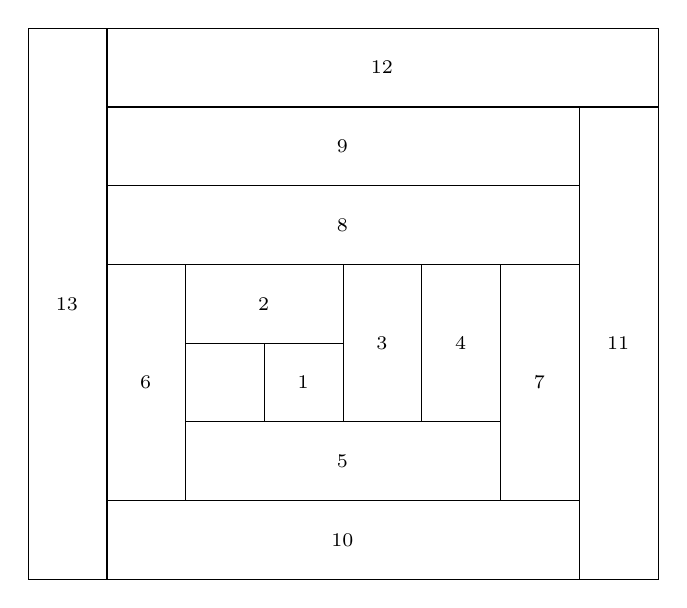
\begin{tikzpicture}[scale=1]
      \draw (1,1) rectangle (2,2) node[pos=0.5]{$\C$};
      \draw (2,1) rectangle (3,2) node[pos=0.5]{$\M_1$};
      \draw (1,2) rectangle (3,3) node[pos=0.5]{$\M_2$};
      \draw (3,1) rectangle (4,3) node[pos=0.5]{$\M_3$};
      \draw (4,1) rectangle (5,3) node[pos=0.5]{$\M_4$};
      \draw (1,0) rectangle (5,1) node[pos=0.5]{$\M_5$};
      \draw (0,0) rectangle (1,3) node[pos=0.5]{$\M_6$};
      \draw (5,0) rectangle (6,3) node[pos=0.5]{$\M_7$};
      \draw (0,3) rectangle (6,4) node[pos=0.5]{$\M_8$};
      \draw (0,4) rectangle (6,5) node[pos=0.5]{$\M_9$};
      \draw (0,-1) rectangle (6,0) node[pos=0.5]{$\M_{10}$};
      \draw (6,-1) rectangle (7,5) node[pos=0.5]{$\M_{11}$};
      \draw (0,5) rectangle (7,6) node[pos=0.5]{$\M_{12}$};
      \draw (-1,-1) rectangle (0,6) node[pos=0.5]{$\M_{13}$};
    \end{tikzpicture}
    \caption{An example of unrestricted iterative juxtaposition of thirteen monotone classes $\M_1,\ldots,\M_{13}$ onto a context-free class $\C$.}
    \label{fig:juxtopia}
  \end{center}
\end{figure}


The one major direction of research that suggests itself after our work is the generalisation to juxtapositions from all four sides: top, bottom, right, and left. See Figure~\ref{fig:juxtopia}. This would require tracking all four extremal points in the permutation. This in itself is not an easy task, as it would require two mutually dependent combinatorial specifications. One that tracks the vertical position of points and the other one that tracks their horizontal positions. Both horizontal and vertical positions of each point are needed to deal with top and side juxtapositions. Assuming we can deal with that, it still remains to determine how to uniquely grid any one given permutation (provided that it is griddable into a given class).

% The problems with gridding arise, for instance, when two classes meet at a corner in a continuous way. Imagine a two-sided juxtaposition as in Figure~\ref{fig:screwyou}. It is of the form shown in Figure~\ref{fig:juxtopia}, but no matter how we do the gridding (first from the side, then from the top; or vice versa), it is not straightforward how to phrase the overlap of two points at the boundary (think along the lines of the rightmost point in the left cell being above the leftmost point in the right cell). This would not be the case in Figure~\ref{fig:screwyou}. On the bright side, one can notice that there are no cycles when juxtaposing from both the top and the side.

% \begin{figure}[ht!]
%   \begin{center}
%     \begin{tikzpicture}[scale=1]
%       \draw (1,3) rectangle (3,5);
%       \draw (1,1) rectangle (3,3) node[pos=0.5]{$\C$};
%       \draw (3,1) rectangle (5,3);
%       \foreach \i in {1,...,40}
%       {
%         \filldraw[black] (1+0.1*\i,5-0.1*\i) circle (0.5pt);
%       }
%       % \filldraw[black] (-0.2,14.6) circle (1.5pt) node[right]{$w$};
%       % \filldraw[black] (-5.4,9.4) circle (1.5pt) node[right]{$z$};
    
%     \end{tikzpicture}
%     \caption{An example of a problematic juxtaposition from both the top and the side.}
%     \label{fig:screwyou}
%   \end{center}
% \end{figure}

Notice that the grid classes like the one in Figure~\ref{fig:juxtopia} contain all acyclic grid classes with one context-free cell. Therefore, a result along the lines of Theorem~\ref{thm:iterjuxt_main} about these acyclic classes is among the goals of our continued work in this area. Another natural question is whether the respective results translate to regular class $\C$ juxtaposed with monotone classes, i.e. are such juxtapositions regular? Do they have rational generating functions?

Finally, we would like to point out that a context-free class $\C$ was chosen because it is a ``nicely behaved'' object to juxtapose monotone classes next to. However, other objects --- maybe more general ones --- could be manageable under favourable circumstances. It remains a direction to pursue. 


